\documentclass[10pt,a4paper,oneside]{article}
%NOTE: This report format is 
\renewcommand{\familydefault}{\sfdefault}
\usepackage[T1,OT1]{fontenc}
\usepackage{multicol}
\usepackage{lipsum}
\usepackage{float}
\usepackage{siunitx}
\usepackage{wrapfig}
\usepackage{setspace}
% \usepackage[document]{ragged2e}
\singlespacing
\newcommand{\hsc}[1]{{\normalsize\MakeUppercase{#1}}}
% \usepackage{geometry}
% \geometry{top=1.5cm,bottom=1.5cm}


\newcommand{\reporttitle}{Pacman Line Following Robot: Technical Report}
\newcommand{\reportauthorOne}{Amal \textbf{C\hsc{HANDRA} - acha932}}
\newcommand{\cidOne}{890345562}
\newcommand{\reportauthorTwo}{Dylan \textbf{F\hsc U - dfu987}}
\newcommand{\cidTwo}{165746216}
\newcommand{\reportauthorThree}{Quentin \textbf{H\hsc{ENG} - qhen143}}
\newcommand{\cidThree}{775834627}
\newcommand{\reportauthorFour}{Louis \textbf{P\hsc{IENAAR} - lpie601}}
\newcommand{\cidFour}{488462824}
\newcommand{\reporttype}{Coursework}
\bibliographystyle{plain}

% include files that load packages and define macros
%%%%%%%%%%%%%%%%%%%%%%%%%%%%%%%%%%%%%%%%%
% University Assignment Title Page 
% LaTeX Template
% Version 1.0 (27/12/12)
%
% This template has been downloaded from:
% http://www.LaTeXTemplates.com
%
% Original author:
% WikiBooks (http://en.wikibooks.org/wiki/LaTeX/Title_Creation)
%
% License:
% CC BY-NC-SA 3.0 (http://creativecommons.org/licenses/by-nc-sa/3.0/)
% 
% Instructions for using this template:
% This title page is capable of being compiled as is. This is not useful for 
% including it in another document. To do this, you have two options: 
%
% 1) Copy/paste everything between \begin{document} and \end{document} 
% starting at \begin{titlepage} and paste this into another LaTeX file where you 
% want your title page.
% OR
% 2) Remove everything outside the \begin{titlepage} and \end{titlepage} and 
% move this file to the same directory as the LaTeX file you wish to add it to. 
% Then add \input{./title_page_1.tex} to your LaTeX file where you want your
% title page.
%
%----------------------------------------------------------------------------------------
%	PACKAGES AND OTHER DOCUMENT CONFIGURATIONS
%----------------------------------------------------------------------------------------
\usepackage{ifxetex}
\usepackage{textpos}
\usepackage{natbib}
\usepackage{kpfonts}
\usepackage[letterpaper,hmargin=2.4cm,vmargin=1.7cm,includeheadfoot]{geometry}
\usepackage{ifxetex}
\usepackage{stackengine}
\usepackage{tabularx,longtable,multirow,subfigure,caption}%hangcaption
\usepackage{fncylab} %formatting of labels
\usepackage{fancyhdr}
\usepackage{color}
\usepackage[tight,ugly]{units}
\usepackage{url}
\usepackage{float}
\usepackage[english]{babel}
\usepackage{amsmath}
\usepackage{graphicx}
\usepackage[colorinlistoftodos]{todonotes}
\usepackage{dsfont}
\usepackage{epstopdf} % automatically replace .eps with .pdf in graphics
\usepackage{natbib}
\usepackage{backref}
\usepackage{array}
\usepackage{latexsym}
\usepackage{etoolbox}

\usepackage{enumerate} % for numbering with [a)] format 



\ifxetex
\usepackage{fontspec}
\setmainfont[Scale=.8]{OpenDyslexic-Regular}
\else
\usepackage[pdftex,pagebackref,hypertexnames=false,colorlinks]{hyperref} % provide links in pdf
\hypersetup{pdftitle={},
  pdfsubject={}, 
  pdfauthor={\reportauthorOne},
  pdfkeywords={}, 
  pdfstartview=FitH,
  pdfpagemode={UseOutlines},% None, FullScreen, UseOutlines
  bookmarksnumbered=true, bookmarksopen=true, colorlinks,
    citecolor=black,%
    filecolor=black,%
    linkcolor=black,%
    urlcolor=black}
\usepackage[all]{hypcap}
\fi

\usepackage{tcolorbox}

% various theorems
\usepackage{ntheorem}
\theoremstyle{break}
\newtheorem{lemma}{Lemma}
\newtheorem{theorem}{Theorem}
\newtheorem{remark}{Remark}
\newtheorem{definition}{Definition}
\newtheorem{proof}{Proof}

% example-environment
\newenvironment{example}[1][]
{ 
\vspace{4mm}
\noindent\makebox[\linewidth]{\rule{\hsize}{1.5pt}}
\textbf{Example #1}\\
}
{ 
\noindent\newline\makebox[\linewidth]{\rule{\hsize}{1.0pt}}
}



%\renewcommand{\rmdefault}{pplx} % Palatino
% \renewcommand{\rmdefault}{put} % Utopia

\ifxetex
\else
\renewcommand*{\rmdefault}{bch} % Charter
\renewcommand*{\ttdefault}{cmtt} % Computer Modern Typewriter
%\renewcommand*{\rmdefault}{phv} % Helvetica
%\renewcommand*{\rmdefault}{iwona} % Avant Garde
\fi

\setlength{\parindent}{0em}  % indentation of paragraph

\setlength{\headheight}{14.5pt}
\pagestyle{fancy}
% \fancyfoot[ER,OL]{\thepage}%Page no. in the left on
                                %odd pages and on right on even pages
% \fancyfoot[OC,EC]{\sffamily }
\renewcommand{\headrulewidth}{0.1pt}
\renewcommand{\footrulewidth}{0.1pt}
\captionsetup{margin=10pt,font=small,labelfont=bf}


%--- chapter heading

\def\@makechapterhead#1{%
  \vspace*{10\p@}%
  {\parindent \z@ \raggedright %\sffamily
        %{\Large \MakeUppercase{\@chapapp} \space \thechapter}
        %\\
        %\hrulefill
        %\par\nobreak
        %\vskip 10\p@
    \interlinepenalty\@M
    \Huge \bfseries 
    \thechapter \space\space #1\par\nobreak
    \vskip 30\p@
  }}

%---chapter heading for \chapter*  
\def\@makeschapterhead#1{%
  \vspace*{10\p@}%
  {\parindent \z@ \raggedright
    \sffamily
    \interlinepenalty\@M
    \Huge \bfseries  
    #1\par\nobreak
    \vskip 30\p@
  }}
  



% %%%%%%%%%%%%% boxit
\def\Beginboxit
   {\par
    \vbox\bgroup
	   \hrule
	   \hbox\bgroup
		  \vrule \kern1.2pt %
		  \vbox\bgroup\kern1.2pt
   }

\def\Endboxit{%
			      \kern1.2pt
		       \egroup
		  \kern1.2pt\vrule
		\egroup
	   \hrule
	 \egroup
   }	

\newenvironment{boxit}{\Beginboxit}{\Endboxit}
\newenvironment{boxit*}{\Beginboxit\hbox to\hsize{}}{\Endboxit}



\allowdisplaybreaks

\makeatletter
\newcounter{elimination@steps}
\newcolumntype{R}[1]{>{\raggedleft\arraybackslash$}p{#1}<{$}}
\def\elimination@num@rights{}
\def\elimination@num@variables{}
\def\elimination@col@width{}
\newenvironment{elimination}[4][0]
{
    \setcounter{elimination@steps}{0}
    \def\elimination@num@rights{#1}
    \def\elimination@num@variables{#2}
    \def\elimination@col@width{#3}
    \renewcommand{\arraystretch}{#4}
    \start@align\@ne\st@rredtrue\m@ne
}
{
    \endalign
    \ignorespacesafterend
}
\newcommand{\eliminationstep}[2]
{
    \ifnum\value{elimination@steps}>0\leadsto\quad\fi
    \left[
        \ifnum\elimination@num@rights>0
            \begin{array}
            {@{}*{\elimination@num@variables}{R{\elimination@col@width}}
            |@{}*{\elimination@num@rights}{R{\elimination@col@width}}}
        \else
            \begin{array}
            {@{}*{\elimination@num@variables}{R{\elimination@col@width}}}
        \fi
            #1
        \end{array}
    \right]
    & 
    \begin{array}{l}
        #2
    \end{array}
    &%                                    moved second & here
    \addtocounter{elimination@steps}{1}
}
\makeatother

%% Fast macro for column vectors
\makeatletter  
\def\colvec#1{\expandafter\colvec@i#1,,,,,,,,,\@nil}
\def\colvec@i#1,#2,#3,#4,#5,#6,#7,#8,#9\@nil{% 
  \ifx$#2$ \begin{bmatrix}#1\end{bmatrix} \else
    \ifx$#3$ \begin{bmatrix}#1\\#2\end{bmatrix} \else
      \ifx$#4$ \begin{bmatrix}#1\\#2\\#3\end{bmatrix}\else
        \ifx$#5$ \begin{bmatrix}#1\\#2\\#3\\#4\end{bmatrix}\else
          \ifx$#6$ \begin{bmatrix}#1\\#2\\#3\\#4\\#5\end{bmatrix}\else
            \ifx$#7$ \begin{bmatrix}#1\\#2\\#3\\#4\\#5\\#6\end{bmatrix}\else
              \ifx$#8$ \begin{bmatrix}#1\\#2\\#3\\#4\\#5\\#6\\#7\end{bmatrix}\else
                 \PackageError{Column Vector}{The vector you tried to write is too big, use bmatrix instead}{Try using the bmatrix environment}
              \fi
            \fi
          \fi
        \fi
      \fi
    \fi
  \fi 
}  
\makeatother

\robustify{\colvec}

%%% Local Variables: 
%%% mode: latex
%%% TeX-master: "notes"
%%% End: 
 % various packages needed for maths etc.
% quick way of adding a figure
\newcommand{\fig}[3]{
 \begin{center}
 \scalebox{#3}{\includegraphics[#2]{#1}}
 \end{center}
}

%\newcommand*{\point}[1]{\vec{\mkern0mu#1}}
\newcommand{\ci}[0]{\perp\!\!\!\!\!\perp} % conditional independence
\newcommand{\point}[1]{{#1}} % points 
\renewcommand{\vec}[1]{{\boldsymbol{{#1}}}} % vector
\newcommand{\mat}[1]{{\boldsymbol{{#1}}}} % matrix
\newcommand{\R}[0]{\mathds{R}} % real numbers
\newcommand{\Z}[0]{\mathds{Z}} % integers
\newcommand{\N}[0]{\mathds{N}} % natural numbers
\newcommand{\nat}[0]{\mathds{N}} % natural numbers
\newcommand{\Q}[0]{\mathds{Q}} % rational numbers
\ifxetex
\newcommand{\C}[0]{\mathds{C}} % complex numbers
\else
\newcommand{\C}[0]{\mathds{C}} % complex numbers
\fi
\newcommand{\tr}[0]{\text{tr}} % trace
\renewcommand{\d}[0]{\mathrm{d}} % total derivative
\newcommand{\inv}{^{-1}} % inverse
\newcommand{\id}{\mathrm{id}} % identity mapping
\renewcommand{\dim}{\mathrm{dim}} % dimension
\newcommand{\rank}[0]{\mathrm{rk}} % rank
\newcommand{\determ}[1]{\mathrm{det}(#1)} % determinant
\newcommand{\scp}[2]{\langle #1 , #2 \rangle}
\newcommand{\kernel}[0]{\mathrm{ker}} % kernel/nullspace
\newcommand{\img}[0]{\mathrm{Im}} % image
\newcommand{\idx}[1]{{(#1)}}
\DeclareMathOperator*{\diag}{diag}
\newcommand{\E}{\mathds{E}} % expectation
\newcommand{\var}{\mathds{V}} % variance
\newcommand{\gauss}[2]{\mathcal{N}\big(#1,\,#2\big)} % gaussian distribution N(.,.)
\newcommand{\gaussx}[3]{\mathcal{N}\big(#1\,|\,#2,\,#3\big)} % gaussian distribution N(.|.,.)
\newcommand{\gaussBig}[2]{\mathcal{N}\left(#1,\,#2\right)} % see above, but with brackets that adjust to the height of the arguments
\newcommand{\gaussxBig}[3]{\mathcal{N}\left(#1\,|\,#2,\,#3\right)} % see above, but with brackets that adjust to the height of the arguments
\DeclareMathOperator{\cov}{Cov} % covariance (matrix) 
\ifxetex
\renewcommand{\T}[0]{^\top} % transpose
\else
\newcommand{\T}[0]{^\top}
\fi
% matrix determinant
\newcommand{\matdet}[1]{
\left|
\begin{matrix}
#1
\end{matrix}
\right|
}



%%% various color definitions
\definecolor{darkgreen}{rgb}{0,0.6,0}

\newcommand{\blue}[1]{{\color{blue}#1}}
\newcommand{\red}[1]{{\color{red}#1}}
\newcommand{\green}[1]{{\color{darkgreen}#1}}
\newcommand{\orange}[1]{{\color{orange}#1}}
\newcommand{\magenta}[1]{{\color{magenta}#1}}
\newcommand{\cyan}[1]{{\color{cyan}#1}}


% redefine emph
\renewcommand{\emph}[1]{\blue{\bf{#1}}}

% place a colored box around a character
\gdef\colchar#1#2{%
  \tikz[baseline]{%
  \node[anchor=base,inner sep=2pt,outer sep=0pt,fill = #2!20] {#1};
    }%
}%
 % short-hand notation and macros
\setlength{\columnsep}{1cm}

%%%%%%%%%%%%%%%%%%%%%%%%%%%%

\begin{document}
% front page
\begin{titlepage}

\newcommand{\HRule}{\rule{\linewidth}{0.5mm}} % Defines a new command for the horizontal lines, change thickness here


%----------------------------------------------------------------------------------------
%	LOGO SECTION
%----------------------------------------------------------------------------------------



\begin{center} % Center remainder of the page

%----------------------------------------------------------------------------------------
%	HEADING SECTIONS
%----------------------------------------------------------------------------------------


\includegraphics[width = 10cm]{./figures/uoa}\\[1.5cm] 
\textbf{\textsc{\Large CS301 - Design: Hardware Software Systems}}\\[1.0cm] 
{\Large U\hsc{niversity} \hsc{of} A\hsc{uckland}}\\[0.5cm] 
{\large D\hsc{epartment} \hsc{of} E\hsc{lectrical} \hsc{and} C\hsc{omputer} E\hsc{ngineering}}\\[0.95cm] 

%----------------------------------------------------------------------------------------
%	TITLE SECTION
%----------------------------------------------------------------------------------------

\HRule \\[0.4cm]
{ \Large \bfseries \reporttitle}\\ % Title of your document
\HRule \\[1.5cm]
\end{center}
%----------------------------------------------------------------------------------------
%	AUTHOR SECTION
%----------------------------------------------------------------------------------------

%\begin{minipage}{0.4\hsize}
\begin{flushleft} \large
\textit{Authors:}\\
\reportauthorOne~(ID: \cidOne)\\ % Your name
\reportauthorTwo~(ID: \cidTwo)\\ % Your name
\reportauthorThree~(ID: \cidThree)\\ % Your name
\reportauthorFour~(ID: \cidFour)   % Your name
\end{flushleft}
\vspace{4cm}
\makeatletter
% Date: \@date 

\vfill % Fill the rest of the page with whitespace



\makeatother


\end{titlepage}




%%%%%%%%%%%%%%%%%%%%%%%%%%% table of content
%If a table of content is needed, simply uncomment the following lines
% \tableofcontents
% \newpage

%%%%%%%%%%%%%%%%%%%%%%%%%%%% Main document
\begin{multicols}{2}
\section{Abstract}
This report covers the analogue and digital design of our line following robot. The overall project helped us develop core computer systems engineering skills that are commonly utilised in the Research and Development field. There were many design decisions made throughout this project which are documented in detail. In this report you will find analysis of our design decisions, commentary of our design process and information of the final product.

\section{Introduction}
In this project, we are tasked with developing a robot that would traverse a projected map and collect all the available food pellets, akin to that of the 80s classic, PacMan. There were two major components to this project; the analogue design and digital design. For the analogue design, data inputs from the environment needs to be processed into a useful form. On the other hand, the design aspect required us to utilise the outputs of the analogue circuit and develop effective algorithms to navigate the map under different scenarios.
\section{Analogue}

The design of the hardware is needed to interpret the projected maze.  To process the light input from the projector, a surface mount phototransistor (TEMT6200) is utilised to interpret the maze. The maze being projected down has black lines representing the path and the white areas of the maze as the barriers. The aim of the analogue design is to clearly differentiate between the black light and white light that are exposed to the light sensors, and represent them as a digital signal for the PSoC. This will require signal processing in the form of filtering, amplification, rectifying and digitising the signal.

\subsubsection*{Phototransistor Configuration}
A phototransistor can be set up in two configurations: common collector and common emitter configuration (See Appendix B: Figure 1 \& 2). In the common collector configuration, the output signal had better resolution as the different light frequencies were easily differentiated. However, the difference between the peak-to-peak voltages of the black light and white light at 2.13Vpk-pk and 1.79Vpk-pk respectively was very low, making it difficult to differentiate them. On the other hand, the resolution of the output signal in the common emitter configuration is slightly worse. For our application, the signal resolution is not important since there is no need to differentiate between the different light frequencies. We are more interested in having a larger difference in peak-to-peak voltage between the black light and white light at 1.8Vpk-pk and 0.28Vpk-pk respectively. Due to this, the common emitter configuration was chosen for the light sensors to clearly distinguish the black light from the white light of the maze. 
\\The current produced from the light sensor ranges from 7.5uA to 39uA based on the type of light it is exposed to. Due to this, the resistor in series needs to be large enough so that voltage across it, from sensing the black and white light, is distinguishable from each other. The value of 100KOhm was chosen so that the theoretical voltage range of the input signal is between 4.25V to 1.1V.

\subsubsection*{Filter}
In reality, the light sensor will also be subjected to other ambient light sources aside from the projector light in the room. The light sources in the room consists of the projector light, artificial ambient light, and natural ambient light which has a frequency of 120Hz, 100Hz and 0Hz respectively. To obtain the pure signals of the projected map, we need to filter out as much of the ambient light as possible. A high-pass filter with a corner frequency of 10Hz was designed to filter out the DC offset of the signal. 
\\Ideally, we would like to have a corner frequency at 105Hz to filter out the artificial ambient light as well. However, in practice, the filter will have a finite roll-off which means the 100 Hz signal will not be filtered since it is too close to the corner frequency. Also, our desired signal would be too close to the corner frequency, thus our desired signal would also be slightly filtered since the gain of the signal would be 0.707 around the corner frequency. Due to these limitations, we designed our high-pass filter with a corner frequency of 15 Hz instead so that only the DC component would be filtered out whilst maintaining the strength of the desired signal. To get a corner frequency of 15 Hz, we chose a 680KOhm resistor and a 15nF capacitor. Above the corner frequency the capacitor acts as a short circuit, therefore the resistor (R) of the light sensor and the resistor (Rf)  of the filter will act as a voltage divider, thus Rf must be significantly larger than R (See Appendix B: Figure 2). For this reason, we chose Rf to be 680KOhm which is significantly larger than R, so that the effect of the voltage divider is minuscule and our voltage into the filter is largely unchanged. 
\\The filtered signal is relatively small with an amplitude of 140 mV and ~0.8V for black and white light respectively, thus needs amplification. An active high pass filter is needed for the filtering of the DC component and the amplification of the signal. We designed our active high pass filter to have a gain of 5.7 so that our signal would now have a max voltage of 0.8V and 4.56V for black and white light respectively which would allow us to easily differentiate between them. 

\subsubsection*{Analogue vs Digital Output Signal}
The input signals into the PSoC can either be in analogue or digital form. If an analogue signal is passed into the PSoC,  the input voltage will have to be sampled by the PSoC ADC and then converted into a digital form. If a digital signal is passed into the PSoC, the signal processing would occur at real-time where the time delay will be due to the time constant of the circuit. Having a digital input will also dramatically simplify the code so that sampling logic does not need to be implemented. Therefore, the use of a digital signal into the PSoC was chosen to simplify software development. 
\\To implement the digital signal, we could use either a comparator or Schmitt-trigger to create high and low signals based on the analogue input signal.  A circuit using comparator has no hysteresis. As electrical signals are noisy, this can lead to the output signal flickering between high and low output when the input signal is reaching the threshold value. Whereas, a circuit using a Schmitt-trigger will reduce the flickering and lead to a clean transition between high and low outputs. Therefore, the decision was made to use a Schmitt-trigger in our circuit. The output signal from the active high-pass filter has a minimum voltage of 1.2V under white light and a maximum voltage of 0.4V under black light. Therefore, the threshold values selected were 0.6V for the low threshold voltage and 1.0V for the high threshold voltage.

\subsubsection*{Rectifier \& Smoothing Capacitor}
The input into the Schmitt-trigger is a periodic signal that is clipped at 0V. For black light, the signal fluctuates between  0-300mV. While in white light, the signal fluctuates between 0-4.5V. Without additional components, the Schmitt-trigger will flicker between a high and low output under white light. This is an undesirable characteristic as the output we want, should be constant under white light. To solve this issue, we used a rectifier to regulate the voltage so that the voltage was relatively constant and above the high threshold. The values selected for the rectifier were 22nF and 680KOhm, these values were a compromise between having a relatively constant voltage and a small time constant so that the time delay doesn’t majorly impair the reaction time of the robot.
\subsubsection*{Sensor Array}
With our overall circuit complete, the light sensors needs to be positioned so that the robot will be able to navigate the maze under all possible scenarios. These scenarios include when the robot should follow a line and when it reaches events (intersections and dead ends).
\\Based on these scenarios, at the very least, we need two intersection sensors, two line sensors and a center sensor. Two line sensors on each side of the path are required so that the robot will be able to detect when it veers off the path and correct this. Two intersection sensors slightly further apart from the lines sensors are also needed to detect events which the robot will be able to react to. Finally, a center sensor will be needed to handle dead end events. The configurations we considered are seen in Appendix C: Figures 4-6. 
\\In the first configuration, as seen in Figure 4, the turning is simple since we can turn as soon as the intersection sensors are triggered. The distance of the front sensors are around the width of the robot so one of the wheels can be used as a pivot point when turning. The problem with this configuration is that the intersection sensors are too far apart so smaller intersections could not be detected. Additionally, the robot would turn too early when at a dead end due to how far the center sensor is from the center of the robot.
\\In the second array, as seen in Figure 5, the distance between the intersection sensors are shorter so that smaller intersections could be detected. All the sensors are also moved closer to the center to prevent early turning. However, this changes the pivot point for turning, thus we would now need to correctly determine when to turn after detecting the event as opposed to the previous arrangement.
\\Finally, Figure 6 shows our final sensor arrangement that is implemented in our final product. The new arrangement fixes the aforementioned issues. The intersection sensors will now indicate when to turn, right after it has finished detecting an event. The center sensor is also just above the center of the robot so when turning 180 degrees, the robot will start turning at the correct place now. See Appendix D, for visual representation of scenarios.

\subsubsection*{PCB Design}
For the PCB Design we had two mounting options: Through Hole Technology (THT) or Surface Mount Technology (SMT). The larger sizes of THT components, allow for more efficient prototyping, especially when soldering and desoldering components. That means if we need to modify our circuit, we can easily switch the component out or solder additional jumper wires. On the other hand, SMT components are much smaller which gives us more freedom over the placements of the components, especially when the board has size constraints. 
\\This allows us to minimise our track lengths and place our circuitry for each light sensor as close to our desired sensor arrangement as possible, which is vital for the performance of the robot. We decided to utilise SMT because it is standard industry practice due to low cost and efficient PCB design. Additionally, we included four DIP switches, two used for functionality, the other two used for testing. Two of the switches are used to change the mode (shortest path and traversing the map) of the robot and the other two are used to turn on the motor and/or the white tracking LEDS. To minimise the length of the tracks, anything fed into the PSoC was placed close to the male header pins. These include the light sensing circuits, voltage divider for the battery, switches and daughter board pins.

\subsubsection*{Testing \& Verification}
Testing and Verification of analogue design is a very important step in the development of a circuit. Verification is used to validate our theoretical design, whereas testing is used to ensure our design works and produces the outcome we desire. The iterations of our design were verified through hand-calculations and verification tools such as LTSpice, before testing our prototype using the oscilloscope and multimeter. Refer to Appendix E for simulations and oscilloscope measurements of our design.
\\We initially started with us testing different phototransistor configurations. After testing, the common-collector proved more appropriate for our application due to the accentuated voltages of black light and white light. The results of the tests also indicated our analogue design would need to include filtering to extract the signal of interest. 
\\The next phase of our design required us to verify different corner frequencies and gains of our active high-pass filter and check the outcomes. From extensive testing, it was found that changing the corner frequency to filter out the ambient light at 100Hz had no meaningful effect on the purity of the desired signal but would negatively affect the strength of it. Due to this, the next iteration of our filter design only focused on attenuating the DC component instead.
\\For the sensor array, a prototype representing the arrangement of sensors was created so we could test different arrangements and how well they would handle scenarios the robot may encounter. By creating a physical prototype of the arrangement, we could test the turning and intersection logic on the projected map itself.
\\After testing, we found the robot reacted too slow to turning events. The reaction time was improved by reducing the time constant of the circuit. A design with a smaller capacitor and resistor produced a significantly faster response time.

\subsubsection*{Final Circuit Design}
% \vspace{-0.5mm}
The final light sensing circuit  consists of a phototransistor in common-emitter configuration. The output of which, was filtered and amplified by a gain of 5.7 using an active high pass filter to have a signal in the 0-5V operating range and to accentuate the difference of the black and white light. A rectifier and smoothing capacitor with a time constant of 14.96 ms was used to convert the AC signal closer to a DC signal. This was then converted to a digital signal using a Schmitt-trigger to give a logic high output signal for black light and a logic low output signal for white light. The PCB was designed utilising Surface-mount technology with small surface-mount components, as this enabled us to easily place light sensor circuit in the necessary locations of the board according to our sensor array layout. Our final circuit design can be seen in Appendix B: Figure 3.
\end{multicols}
\newpage
\begin{multicols}{2}
\section{Digital}
\subsubsection*{PWM Motor Control} 
Instead of applying a constant voltage across a DC motor, we repeatedly switch the motor on and off with a fixed voltage applied to the motor. This is done by sending PWM (Pulse Width Modulation) pulses to power the MOSFET in order to turn it on and off. Then, the motor sees the average voltage while it depends on duty cycle of PWM pulses. The speed of rotation is proportion to this average voltage. By PWM method, it’s easier to control the DC motor speed rather than by directly controlling the voltage across it. All we have to do is to modulate pulse width, in other words, a duty cycle. Also, a power MOSFET consumes only negligible power in switching. PSoC has built in PWM modules which allows for simple motor speed control using PWM.

\subsubsection*{Path Finding Algorithms}
To find the path to a particular destination, we considered algorithms such as Breadth First Search (BFS), Depth First Search (DFS), Dijkstra’s algorithm and the A* algorithm.
\\DFS is a traversal algorithm that uses the idea of backtracking. It involves exhaustive searches of all the nodes/vertices by going ahead until the depth of the current path is reached, you then backtrack to the previous intersection to find further unvisited nodes to traverse. This is repeated until the destination is found or all nodes have been visited. The problems with DFS are that we can't find the optimal shortest path and that the algorithm leads to subpar performance for our use case. Also, the maze is modelled as an unweighted graph which can contain cycles, we have to ensure that the nodes that are visited are marked to prevent visiting the same node more than once so that it doesn't end up in an infinite loop. Due to the unpredictable nature of DFS, it was used to implement mode one.
\\As the maze is modelled as an unweighted graph, we considered BFS, Dijkstra’s and A* for the finding the shortest path. BFS is a traversal algorithm where you start traversing from a source node and traverse the graph at the present depth thus exploring the neighbour nodes.  You must then move towards the next-level neighbour nodes. This is repeated until the destination node is found. Like DFS, we must ensure that the visited nodes are marked to prevent visiting the same node more than once so that it doesn't end up in an infinite loop. Dijkstra's algorithm functionally is like BFS. The difference between them is the order in which nodes are considered. Where BFS will consider all edges from a single node before moving on to other nodes, while Dijkstra's algorithm will always consider the lowest-weight unseen edge, from the set of edges connected to all nodes that have been seen so far. The A* algorithm is an implementation that extends Dijkstra’s algorithm. However, instead of only using the weight to select which vertices to explore next, A* greedily chooses the next node using the weight (in our case the weight is always one) and a heuristic. For our project the robot can only move in four directions in the maze therefore we chose an admissible heuristic in the Manhattan distance as our heuristic function. BFS has a time complexity of $O(V+E)$, Dijkstra's has a time complexity of $O(V^2)$ and A* has a time complexity of $O(E)$ where V and E are the vertices and edges in the graph respectively. Therefore, for mode two, the A* algorithm was used.
\\For both mode one and two, the robot then utilises these algorithms to map out the entire path it will travel to collect all the pellets. The nodes of the entire path are then stored in an array. Refer to Appendix F, for more details about the algorithms.


\subsubsection*{Line Following Method}
To follow a line, two line sensors are used. Initially, our method for following a line would involve reversing the polarity of one wheel when the line sensor of the same side started to veer into the black line. This meant our forward movement was jittery due to the wheels swinging back and forth, which ultimately caused issues when turning due to entering intersections on an angle . Our new method adjusts the PWM of one wheel by a set value instead. This allowed for a smoother motion, fixing our aforementioned issue with turning. Refer to Appendix F: Figure 27 for more detail.

\subsubsection*{Data structure and Data Management}
Our robot is reliant on the projected map in order to traverse it. Due to this, the overall system is reactive, taking in many processed data inputs from the environment constantly. In order to maximise the computation time and minimise unnecessary resource usage, we thought carefully about the data structures used and  how our data is managed.
\\The main data structure to store our data are 1D and 2D arrays. Alternative data structures were considered such as linked lists or queues. However, an array would be a more sensible option for our application as accessing a specific element has a time complexity of $O(1)$ as opposed to $O(n)$ of a linked list, refer to Appendix A: Table 3. Arrays require less memory, and are quicker to access specific data than the aforementioned data structures. Though arrays are static and require us to know its size during instantiation, we know the size of our data thus only the minimum required memory will be allocated. Also, our implementation does not require us to modify the size of the array, thus we do not need unnecessary features the other data structures offer.
\\The system utilises a PSoC thus it is in our best interest to maximise the use of our limited memory. In terms of data types, the smallest precision was used where appropriate to minimise memory usage. For instance, any flag variables used to signify an event was set as an uint8 data type since we do not need precision beyond 8 bits.

\subsubsection*{RF/Implementation}
In order to implement the algorithms mentioned above, we need to be able to track the position of our robot. However, in our algorithm, we only need to monitor the position of the robot constantly when the robot needs to stop in the middle of a path. In all other cases, we only need to know when the robot reaches an event such as an intersection or dead end. In other words, whilst the RF transmission of our position could improve our accuracy, it is unnecessary in our implementation of traversing. Aside from the additional resources required to process the RF, another problem is that our system would be reliant on RF to reaffirm our position. Ignoring the corner cases where the RF transmission sends incorrect data, the timing of the RF transmission is simply too inconsistent for the rate at which we plan to operate at.

\subsubsection*{Testing \& Verification}
Similar to the analogue design, the algorithms were verified and tested before they were implemented on the robot. For our path finding algorithms, the algorithms were coded in a separate environment and tested before optimising and porting it over to the PSoC Creator environment. By developing the algorithm in a separate environment, we are able to test the code much more efficiently by effectively isolating the algorithm, ensuring the correct path is generated. To test the algorithms, the code was compiled using a Command Line Interface (CLI) thus we are able to log each vital step of the algorithm and confirm it aligns with what we expect. A visual representation of the states can also be printed out for accessibility when testing.
\\Once ported over, we had to implement the path finding algorithms with our robot. This part of the project was difficult due to the need to synchronise the algorithms with the movement of the robot and the light sensing circuits. When unexpected behaviour occurred during testing, we followed a procedure until the problem was found. The purpose of procedure was to ensure testing was as efficient as possible by isolating the problem, using a given hierarchy. The order of the procedure is as follows; Repeat the test a few times, ensure the light sensors are working, and incrementally test the state logic of the code.  The first step ensures the bug can be reproduced thus can be fixed in a reasonable timeframe. The second step verifies that the problem is not a prototyping issue but rather a logic issue. Finally, based on the previous steps, we can infer the problem is indeed a logic issue thus debug the code.
\section{Conclusion}
For this project, we were tasked with designing the analogue and digital aspects of a line following robot. The analogue design required us to interpret the lights projected by the maze and process it into a useful form for the robot. The digital aspect requires us to utilise our light sensing circuits to synchronise the robot’s position with the path finding algorithm and control our motors. With many approaches available, it was up to our team to consider the best solution to implement. Due to this, we have developed skills that are vital to our professional career throughout this project. This project allowed us to explore many aspects of Research \& Development through electronic and software development, which further developed our core engineering skills. Our team dynamic was key to the success of this project as we were able to utilise everyone’s strengths and weaknesses, to produce a final product that we are satisfied with.

\end{multicols}


\newpage
\section{Contributions}
\begin{table}[h]
\centering
\resizebox{\textwidth}{!}{\begin{tabular}{|l|llll|}
\hline
\textbf{Task} & \multicolumn{1}{l|}{\textbf{Amal Chandra}} & \multicolumn{1}{l|}{\textbf{Dylan Fu}} & \multicolumn{1}{l|}{\textbf{Quentin Heng}} & \multicolumn{1}{l|}{\textbf{Louis Pienaar}} \\ \hline
\textbf{Analogue Design} & 22\% & 34\% & 34\% & 10\%                                \\ \cline{1-1}
\textbf{Analogue Testing \& Verification} & 33\% & 33\% & 33\% & 1\%                  \\ \cline{1-1}
\textbf{Assembly} & 60\% & 20\% & 20\% & 0\%                                          \\ \cline{1-1}
\textbf{Path Algorithms} & 5\% & 12.5\% & 12.5\% & 70\%                                   \\ \cline{1-1}
\textbf{Benchmark Tests} & 25\% & 25\% & 25\% & 25\%                                    \\ \cline{1-1}
\textbf{Software Design} & 10\% & 15\% & 15\% & 60\%                                \\ \cline{1-1}
\textbf{Software Testing \& Verification} & 10\% & 25\% & 25\% & 40\%               \\ \cline{1-1}
\textbf{Integration} & 25\% & 25\% & 25\% & 25\%                                    \\ \cline{1-1}
\textbf{Report} & 25\% & 25\% & 25\% & 25\%                                       \\ \hline
\end{tabular}}
% \caption{Table of contributions towards the project}
\end{table}

\section{Appendices}
\subsection*{Appendix: A}
\begin{table}[h!]
\centering
\resizebox{\textwidth}{!}{\begin{tabular}{|l|l|l|l|l|l|l|}
\hline
\textbf{Photo-transistor Configuration}                  & \textbf{Type} & \textbf{Min} & \textbf{Max} & \textbf{Avg} & \textbf{Pk-Pk} & \textbf{Frequency} \\ \hline
\multirow{2}{*}{\textbf{Common Collector}} & \textbf{White} & $1.38V$ & $-1.31V$ & $0.06V$ & $2.13V$ & $120Hz$          \\ \cline{2-7} 
                           & \textbf{Black} & $0.92V$ & $-0.93V$ & $0.06V$ & $2.13V$ & $120Hz$          \\ \hline
\multirow{2}{*}{\textbf{Common Emitter}} & \textbf{White} & $3.7V$ & $1.93V$ & $3V$ & $1.8V$ &  $120Hz$         \\ \cline{2-7} 
                           & \textbf{Black} & $4.46V$ & $4.18V$ & $4.33V$ & $0.28V$ & $120Hz$          \\ \hline
\end{tabular}}
\caption{Voltage comparison using different photo-transistor configurations.}
\end{table}

\begin{table}[h!]
\centering
\resizebox{\textwidth}{!}{\begin{tabular}{|l|l|l|l|l|l|l|}
\hline
\textbf{Light Source}                  & \textbf{Type} & \textbf{Min} & \textbf{Max} & \textbf{Avg} & \textbf{Pk-Pk} & \textbf{Frequency} \\ \hline
\multirow{2}{*}{\textbf{Projector Only}} & \textbf{White} & $4.4V$ & $0.06V$ & $1.6V$ & $4.3V$ & $120Hz$          \\ \cline{2-7} 
                           & \textbf{Black} & $0.38V$ & $0.06V$ & $0.18V$ & $0.32V$ & $120Hz$          \\ \hline
\multirow{2}{*}{\textbf{All Lights On}} & \textbf{White} & $3.4V$ & $0.07V$ & $1.1V$ & $3.1V$ &  $120Hz$         \\ \cline{2-7} 
                           & \textbf{Black} & $0.54V$ & $0.06V$ & $0.02V$ & $0.48V$ & $120Hz$          \\ \hline
\end{tabular}}
\caption{Voltage comparison between black and white light.}
\end{table}

\begin{table}[h!]
\centering
\resizebox{\textwidth}{!}{\begin{tabular}{|l|l|l|l|l|l|l|}
\hline
\textbf{} & \multicolumn{2}{l|}{\textbf{Array}}           & \multicolumn{2}{l|}{\textbf{Linked List}}           & \multicolumn{2}{l|}{\textbf{Queue}}           \\\hline
\textbf{Situation} & \textit{\textbf{Average}} & \textit{\textbf{Worst}} & \textit{\textbf{Average}} & \textit{\textbf{Worst}} & \textit{\textbf{Average}} & \textit{\textbf{Worst}} \\\hline
\textbf{Accessing Element} & $O(1)$ & $O(n)$ & $O(n)$ & $O(n)$ & $O(n)$ & $O(n)$ \\\hline
\textbf{Insertion/Deletion} & $O(n)$ & $O(n)$ & $O(1)$ & $O(1)$ & $O(1)$ &  $O(1)$ \\\hline         
\end{tabular}}
\caption{Time complexity comparison between arrays, linked lists and queues.}
\end{table}

\newpage
\subsection*{Appendix: B}
\begin{multicols}{2}

\begin{figure}[H]
\centering
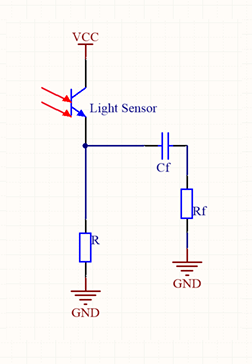
\includegraphics[width=0.4\textwidth]{figures/common-collector}
\caption{Common Collector configuration of the light sensor.}
\end{figure}

\begin{figure}[H]
\centering
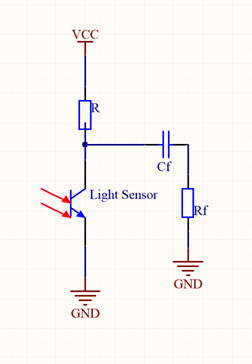
\includegraphics[width=0.4\textwidth]{figures/common-emitter.png}
\caption{Common Emitter configuration of the light sensor.}
\end{figure}
\end{multicols}

\begin{figure}[H]
\centering
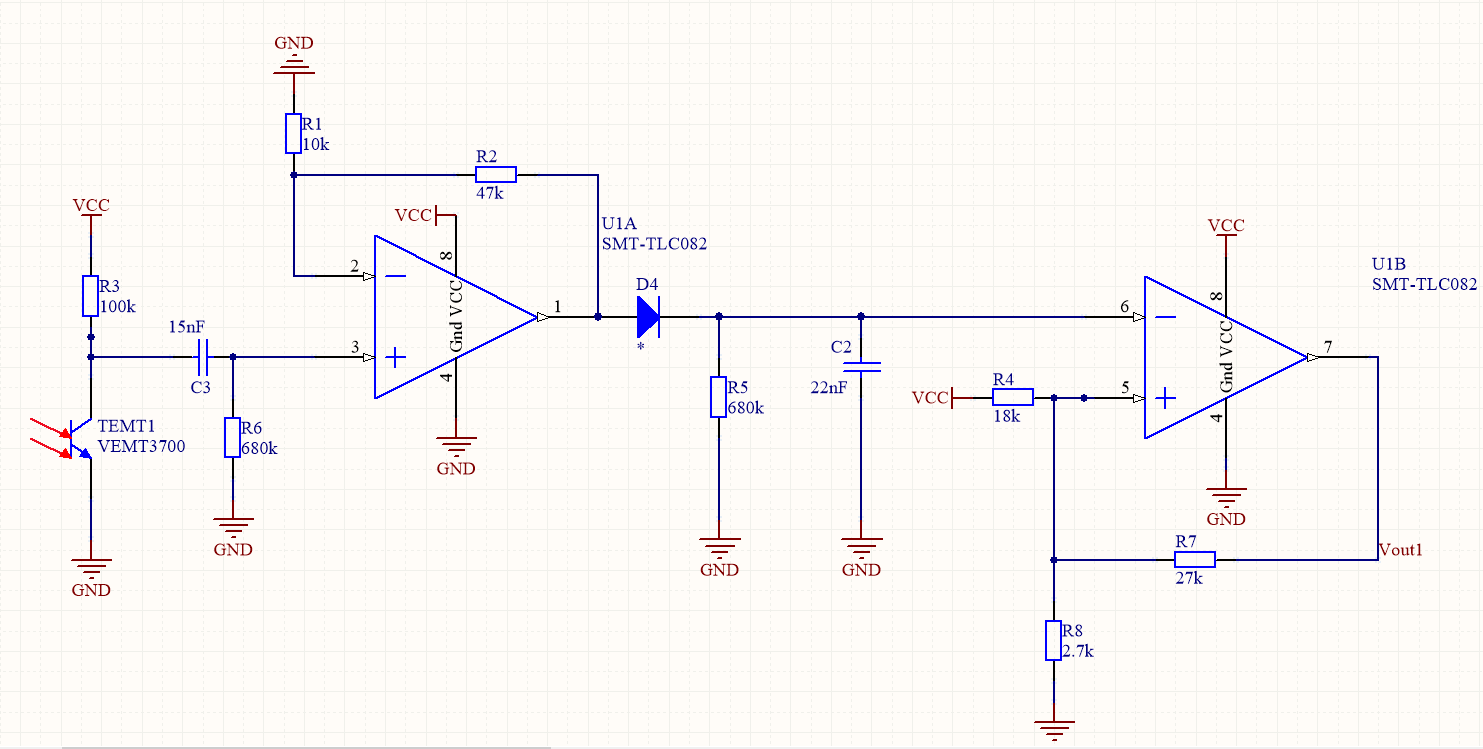
\includegraphics[width=\textwidth]{figures/full-circuit.png}
\caption{Final light sensing circuit design.}
\end{figure}

\subsection*{Appendix: C}

\begin{figure}[H]
\centering
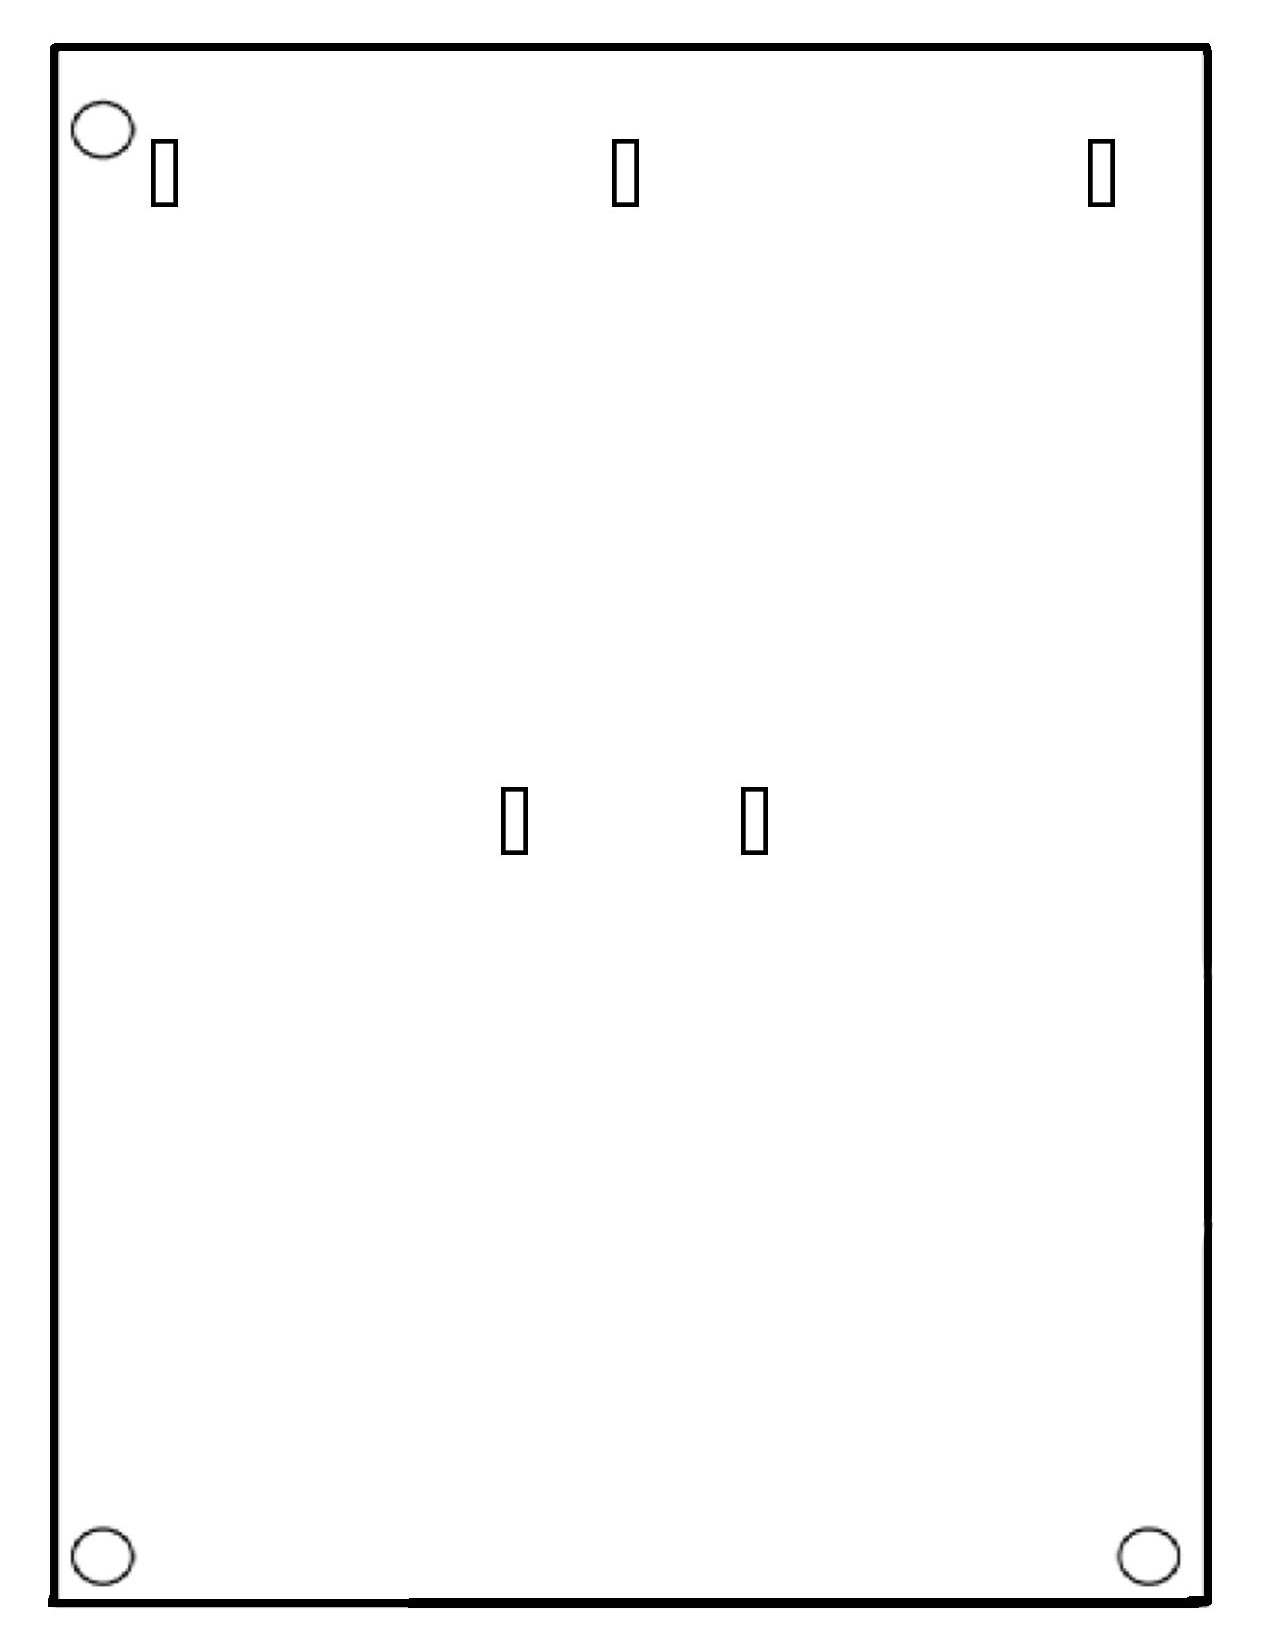
\includegraphics[width=0.95\textwidth]{figures/sarray1.jpg}
\caption{Sensor Arrangement 1.}
\end{figure}


\begin{figure}[H]
\centering
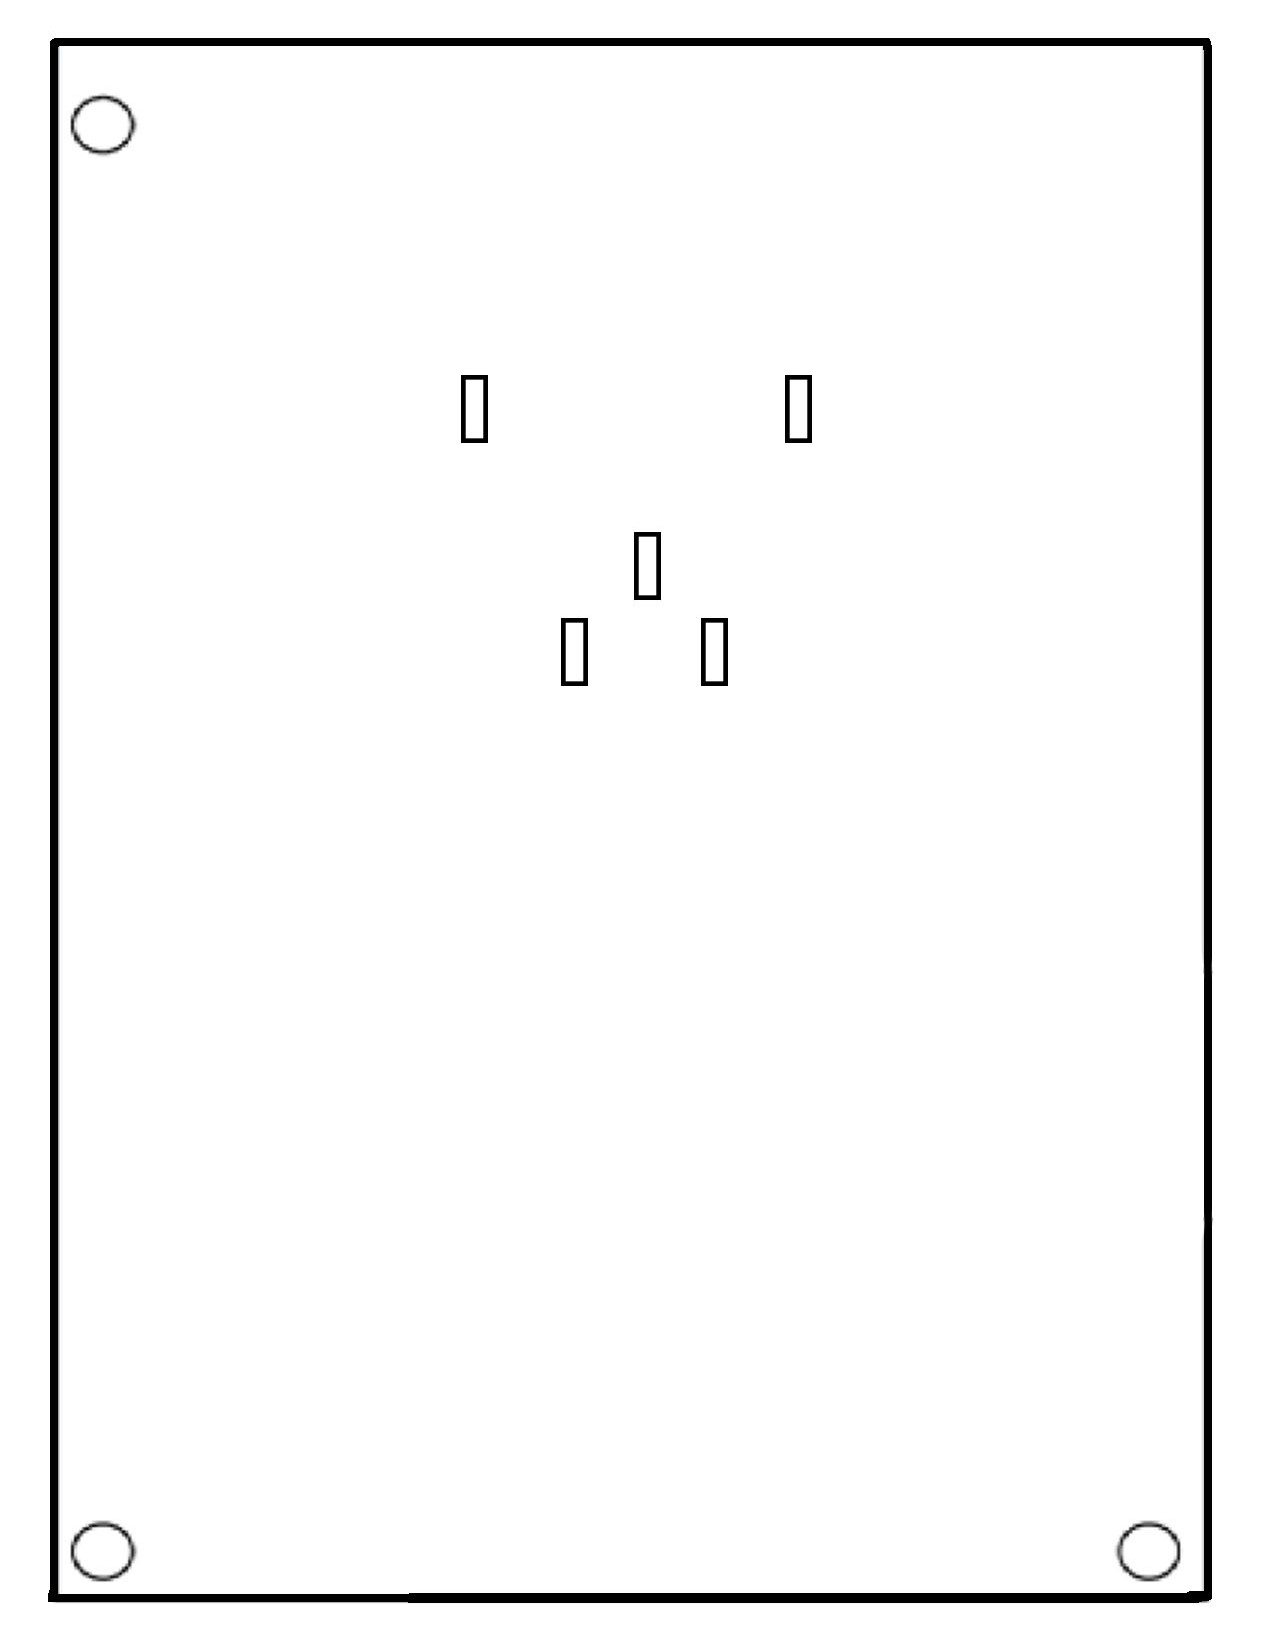
\includegraphics[width=0.95\textwidth]{figures/sarray2.jpg}
\caption{Sensor Arrangement 2.}
\end{figure}

\begin{figure}[H]
\centering
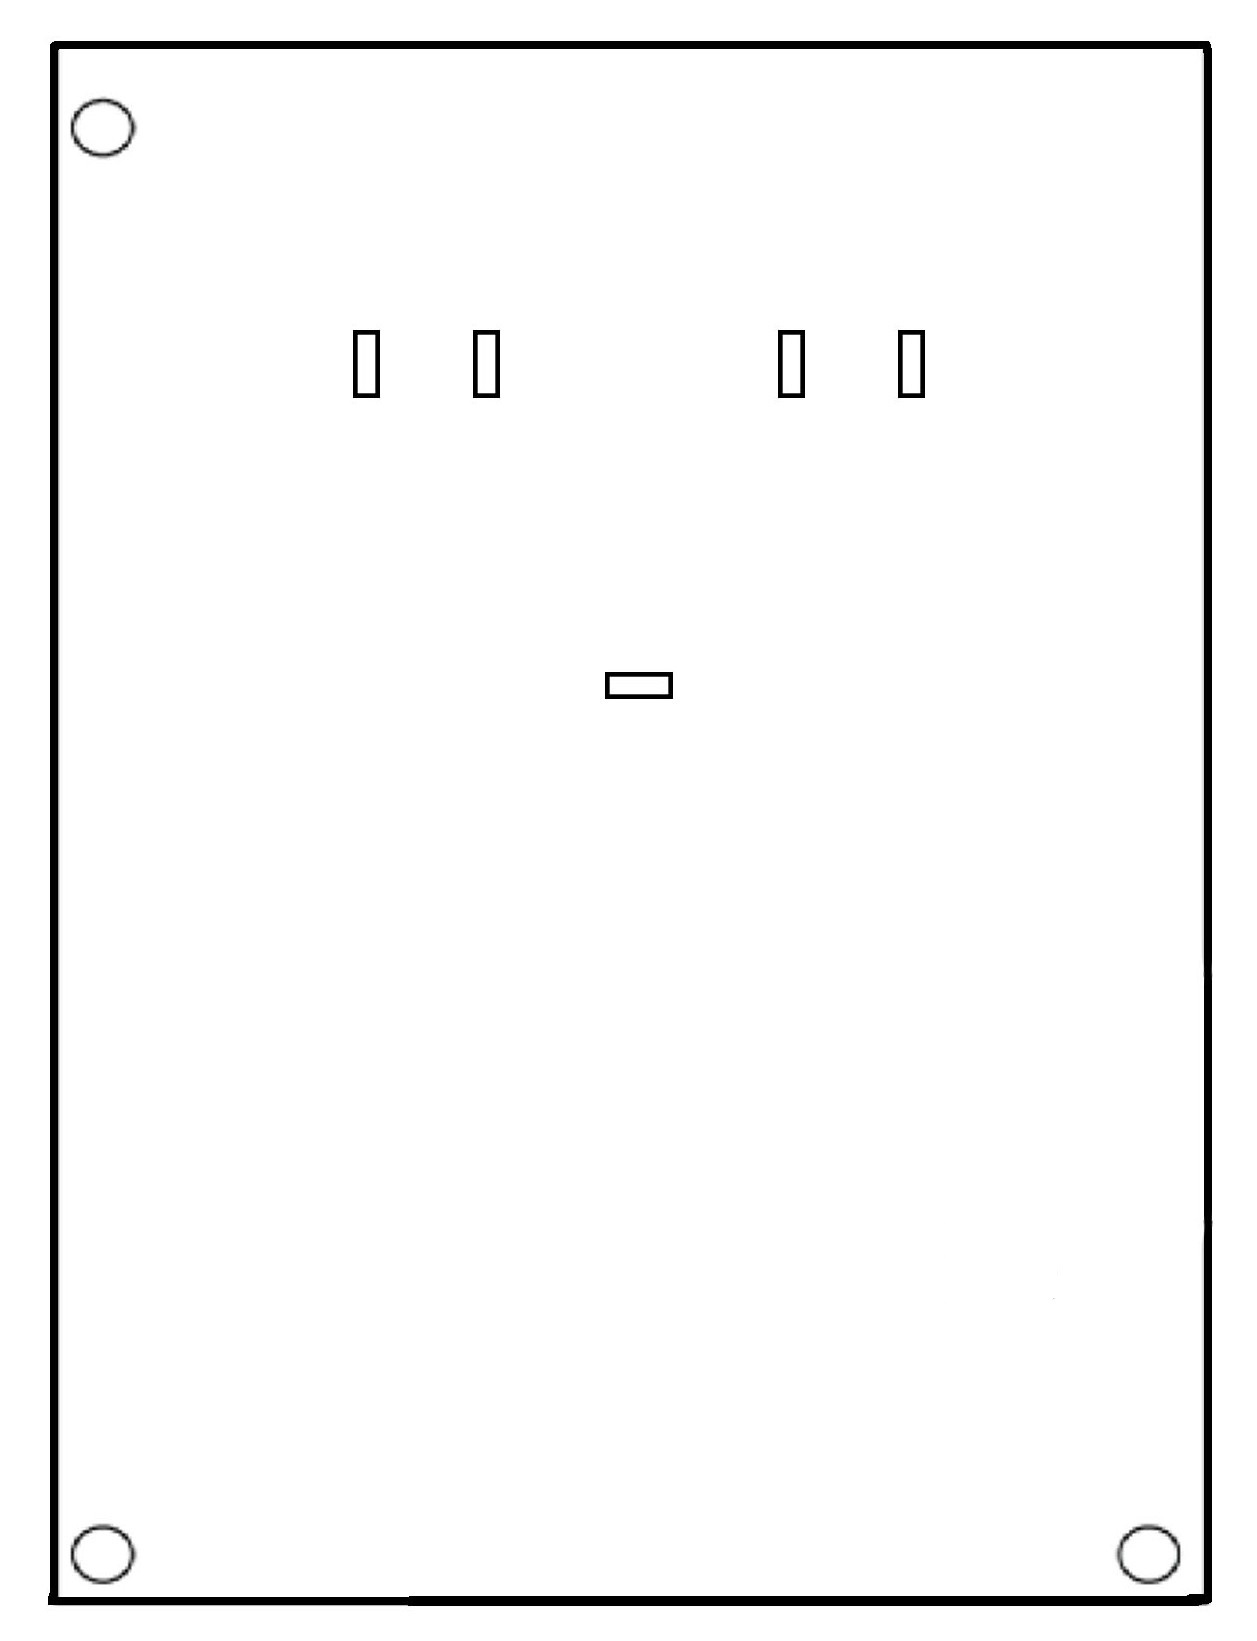
\includegraphics[width=0.95\textwidth]{figures/sarray3.jpg}
\caption{Final Sensor Arrangement.}
\end{figure}

\newpage
\subsection*{Appendix: D}

\begin{multicols}{2}

\begin{figure}[H]
\centering
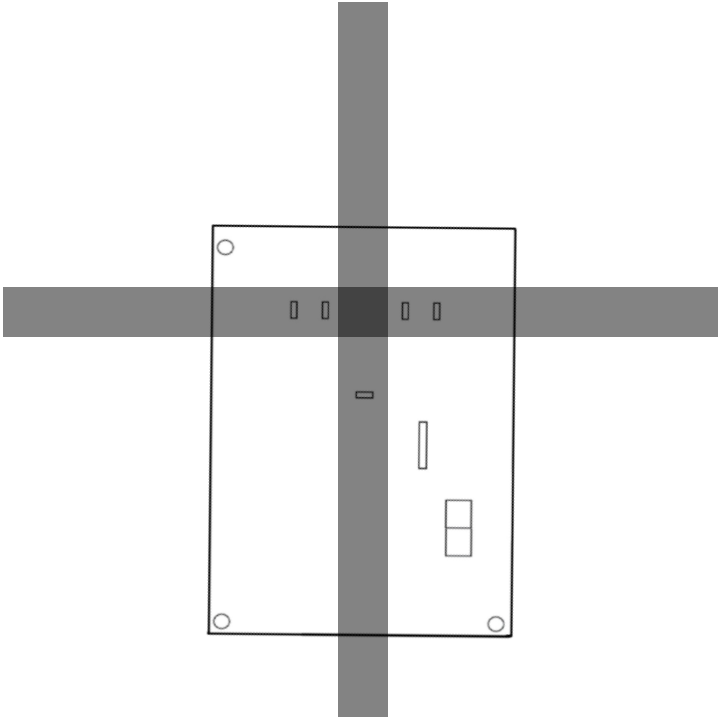
\includegraphics[width=0.3\textwidth]{figures/intersection-1.png}
\caption{Event detected by both Intersection Sensors.}
\end{figure}

\begin{figure}[H]
\centering
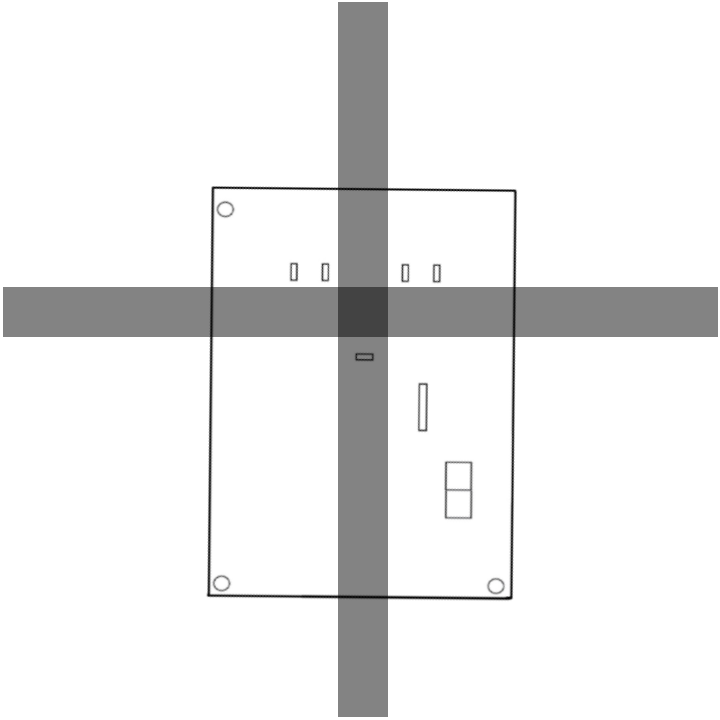
\includegraphics[width=0.3\textwidth]{figures/intersection-2.png}
\caption{Event detection finished, robot will perform appropriate action.}
\end{figure}

\end{multicols}

\begin{multicols}{4}

\begin{figure}[H]
\centering
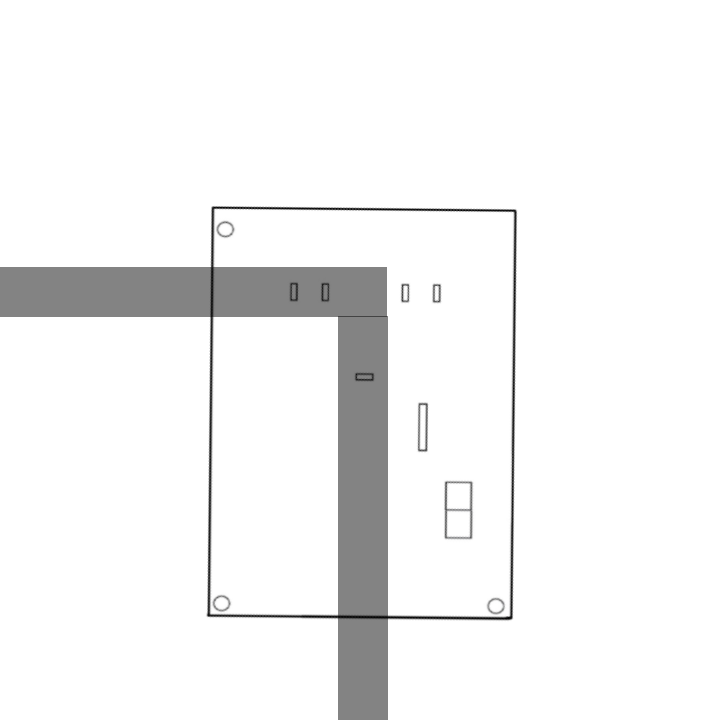
\includegraphics[width=0.2\textwidth]{figures/corner-1.png}
\caption{Event detected by left intersection sensor. Left corner inferred based on internal logic.}
\end{figure}

\begin{figure}[H]
\centering
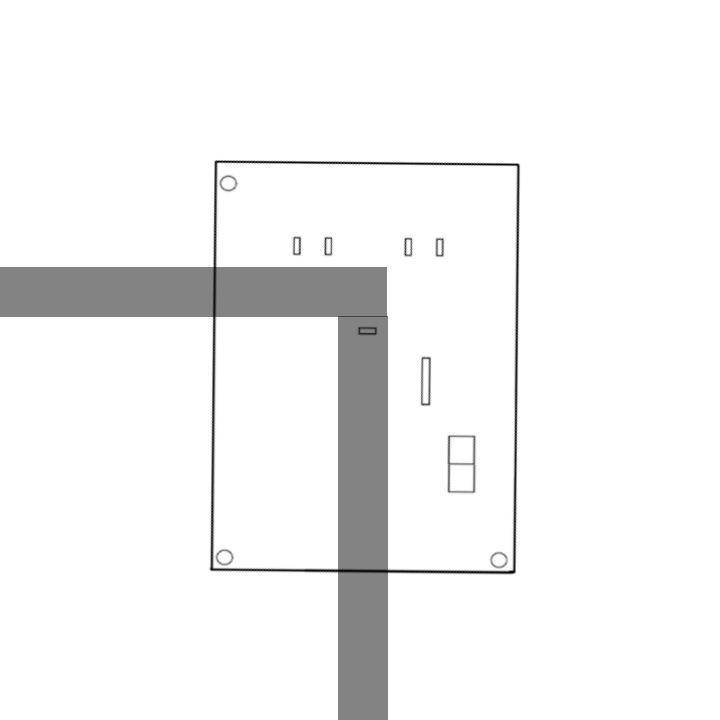
\includegraphics[width=0.2\textwidth]{figures/corner-2.png}
\caption{Event detection finished. Robot will perform appropriate action.}
\end{figure}

\begin{figure}[H]
\centering
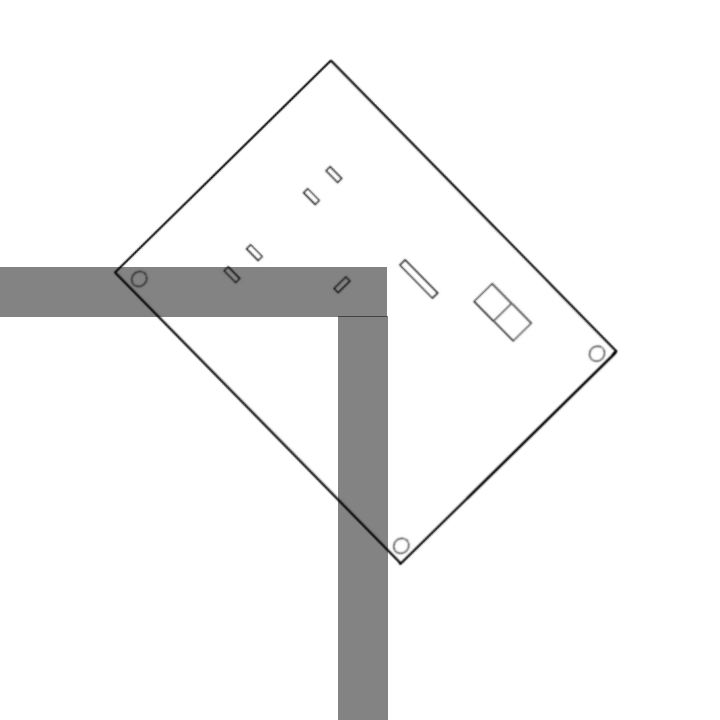
\includegraphics[width=0.2\textwidth]{figures/corner-3.png}
\caption{Robot begins turning here.}
\end{figure}

\begin{figure}[H]
\centering
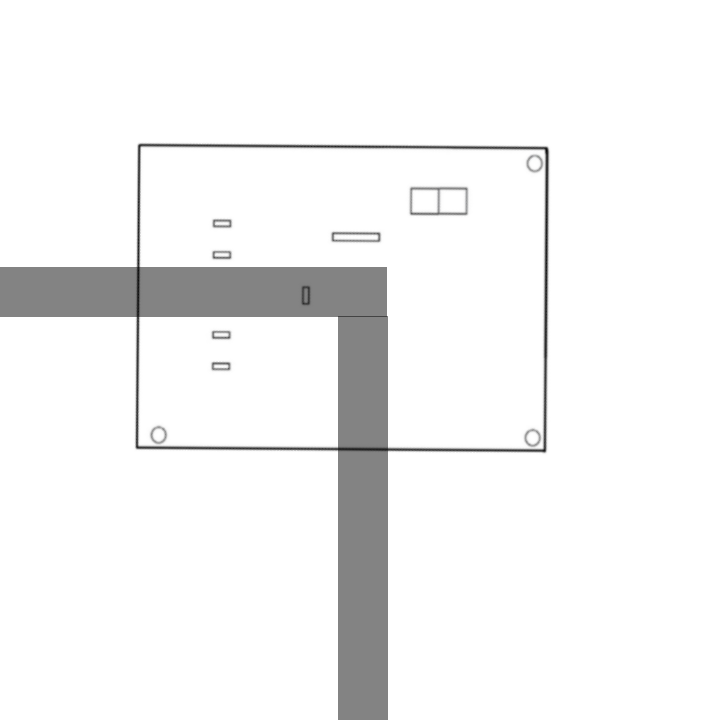
\includegraphics[width=0.2\textwidth]{figures/corner-4.png}
\caption{Robot completes turn. Light sensor return to neutral state.}
\end{figure}

\end{multicols}

\vspace{4mm}

\begin{multicols}{4}

\begin{figure}[H]
\centering
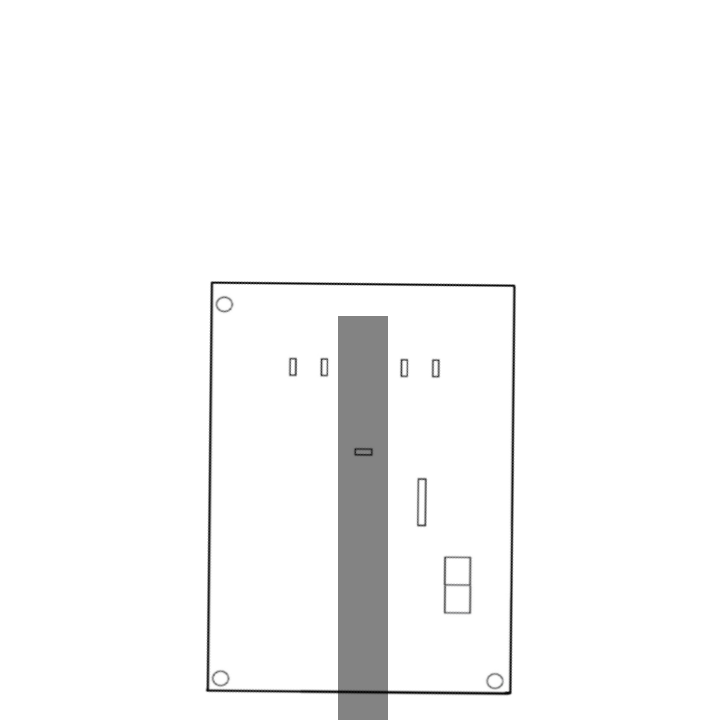
\includegraphics[width=0.2\textwidth]{figures/deadend1.png}
\caption{Center sensor polling for dead end.}
\end{figure}

\begin{figure}[H]
\centering
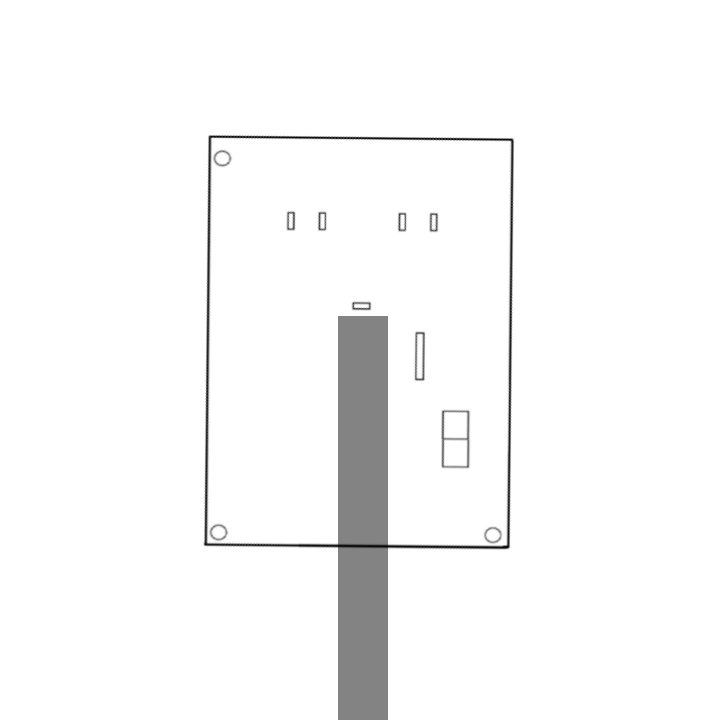
\includegraphics[width=0.2\textwidth]{figures/deadend2.png}
\caption{Center sensor detects event. Dead end inferred from internal logic.}
\end{figure}

\begin{figure}[H]
\centering
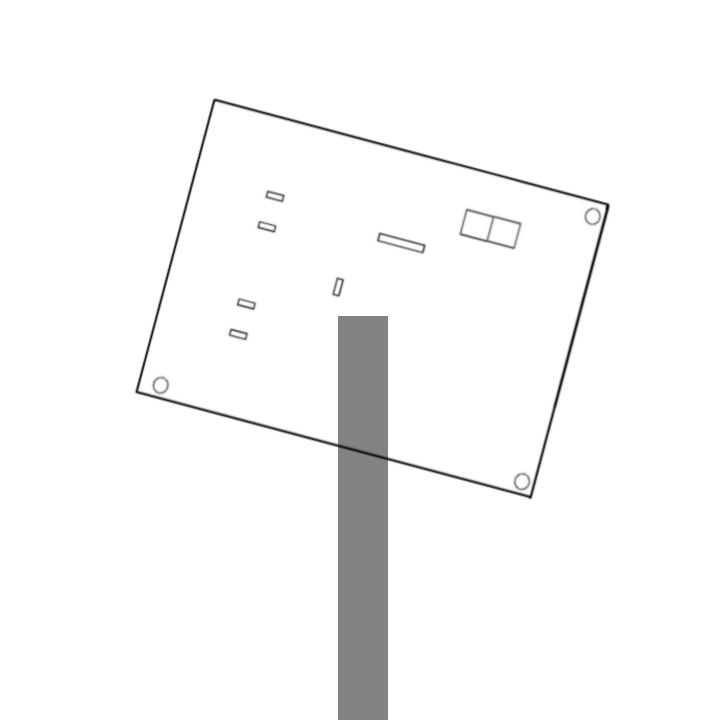
\includegraphics[width=0.2\textwidth]{figures/deadend3.png}
\caption{Robot begins turning here.}
\end{figure}

\begin{figure}[H]
\centering
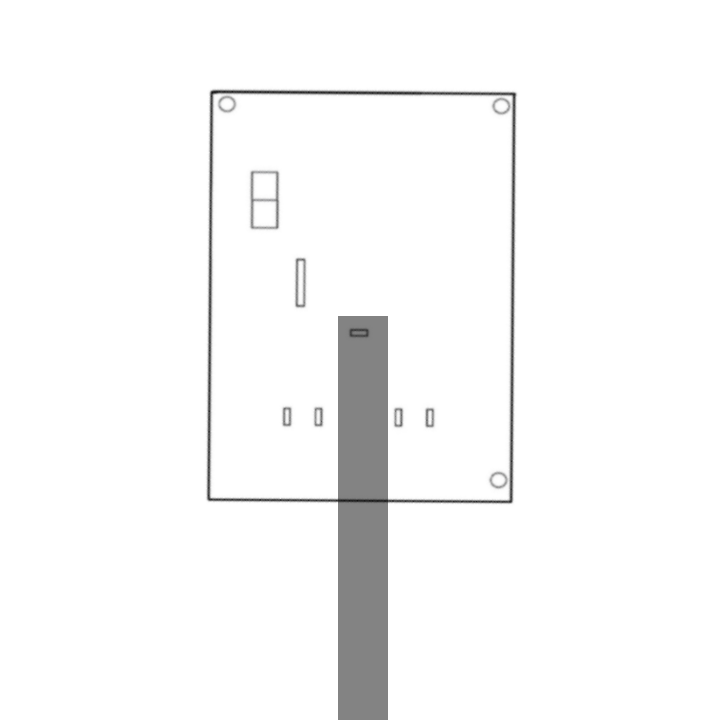
\includegraphics[width=0.2\textwidth]{figures/deadend4.png}
\caption{Robot completes 180 degree turn.}
\end{figure}

\end{multicols}

\subsection*{Appendix: E}

\begin{figure}[H]
\centering
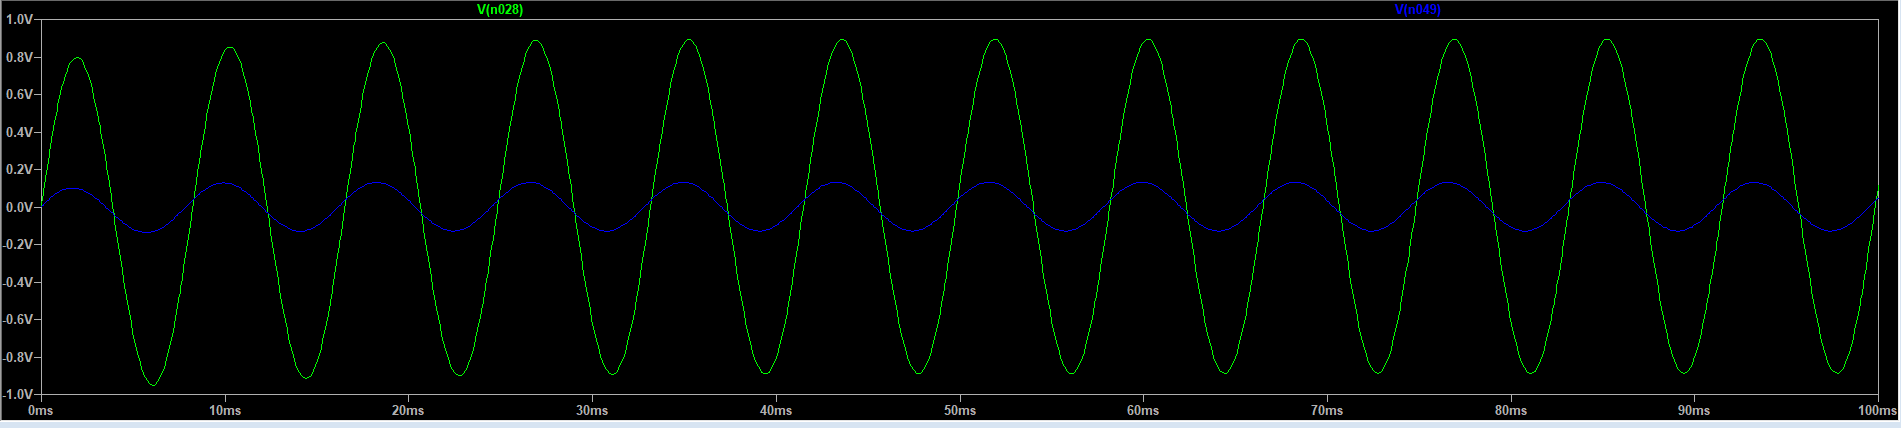
\includegraphics[width=\textwidth]{figures/LTS-filter.PNG}
\caption{LTSpice simulation of the high-pass filter component of the Active high-pass filter.}
\end{figure}

\begin{figure}[H]
\centering
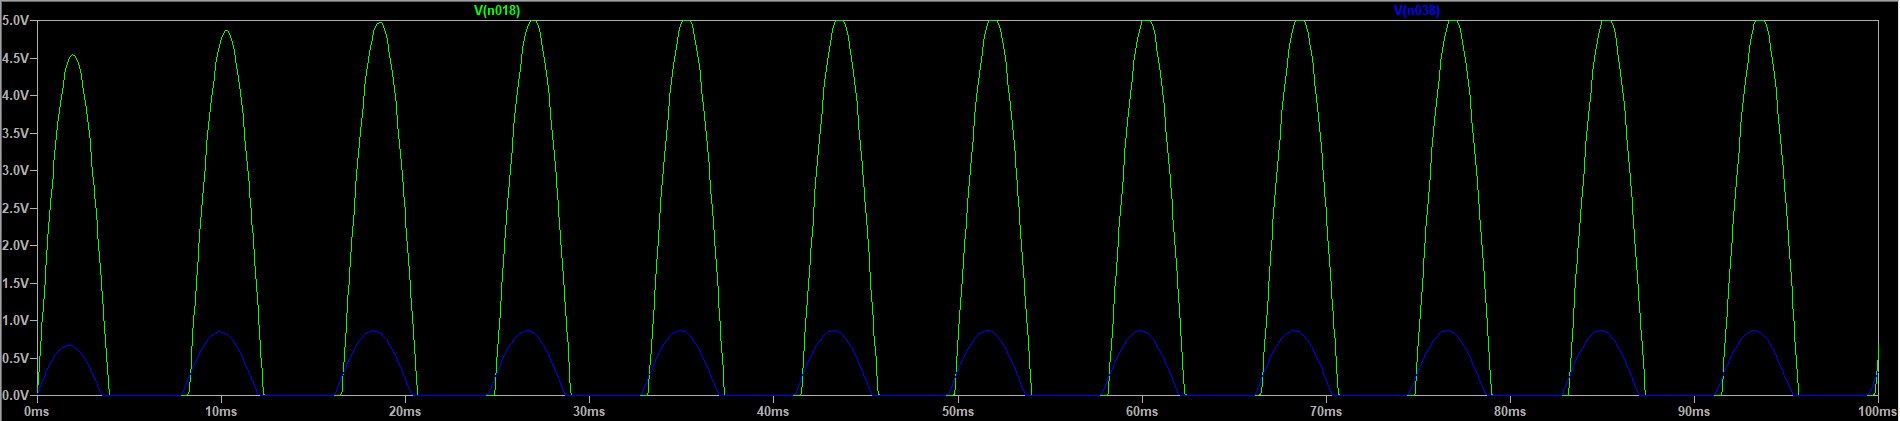
\includegraphics[width=\textwidth]{figures/LTS-gain.PNG}
\caption{LTSpice simulation of the amplification component of the Active high-pass filter.}
\end{figure}

\begin{figure}[H]
\centering
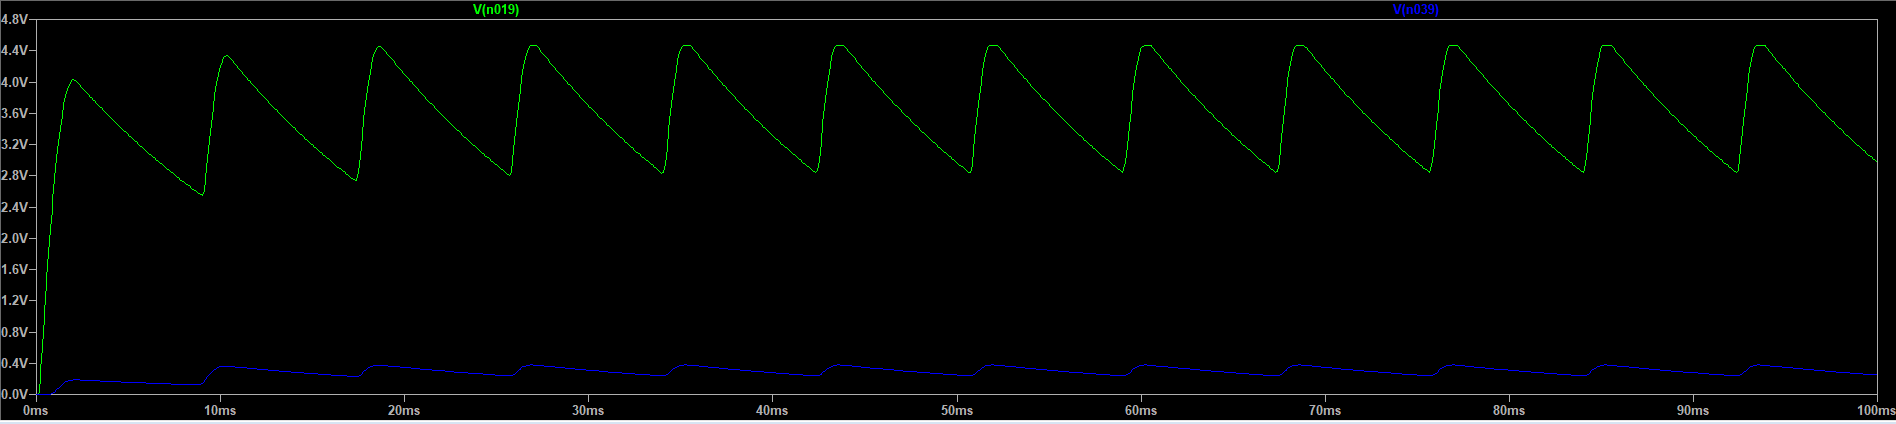
\includegraphics[width=\textwidth]{figures/LTS-rectified.PNG}
\caption{LTSpice simulation of the rectifier and smoothing capacitor output.}
\end{figure}

\begin{figure}[H]
\centering
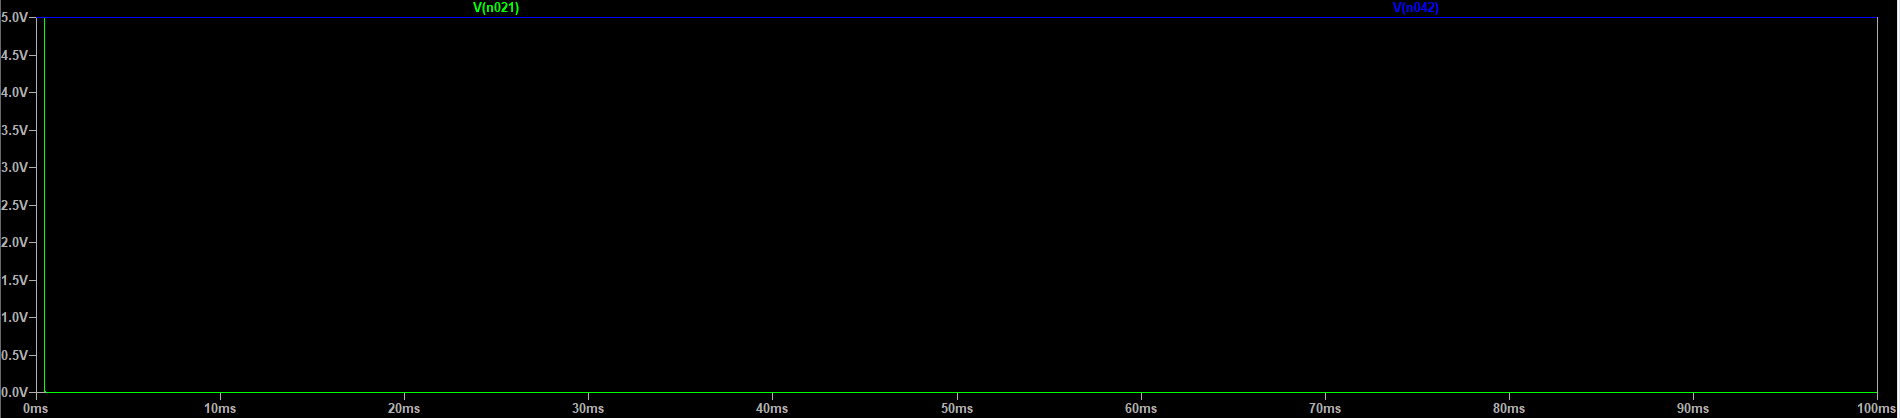
\includegraphics[width=\textwidth]{figures/LTS-output.PNG}
\caption{LTSpice simulation of the Schmitt-trigger output.}
\end{figure}

\begin{figure}[H]
\centering
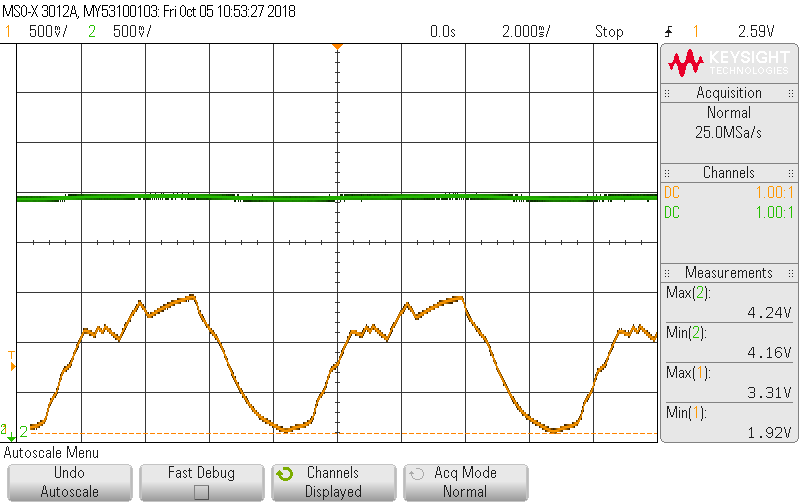
\includegraphics[width=0.9\textwidth]{figures/Osc-ls.png}
\caption{Light sensor output comparison between black and white light.}
\end{figure}

\begin{figure}[H]
\centering
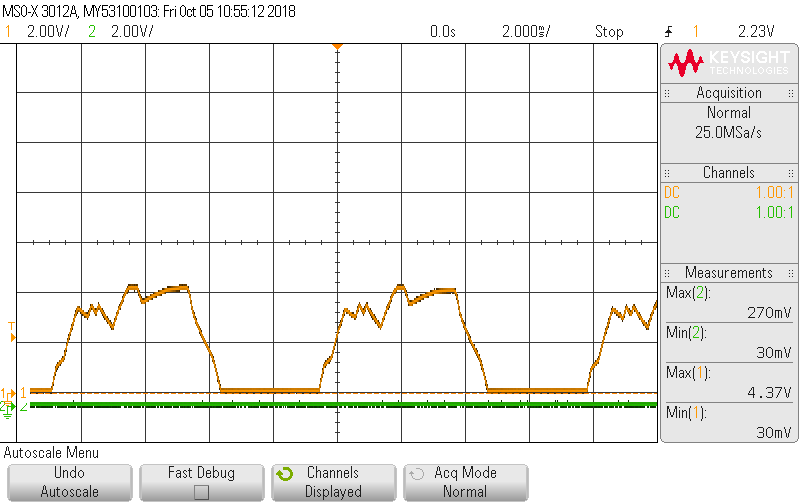
\includegraphics[width=0.9\textwidth]{figures/Osc-filtergain.png}
\caption{Active high-pass filter output comparison between black and white light.}
\end{figure}

\begin{figure}[H]
\centering
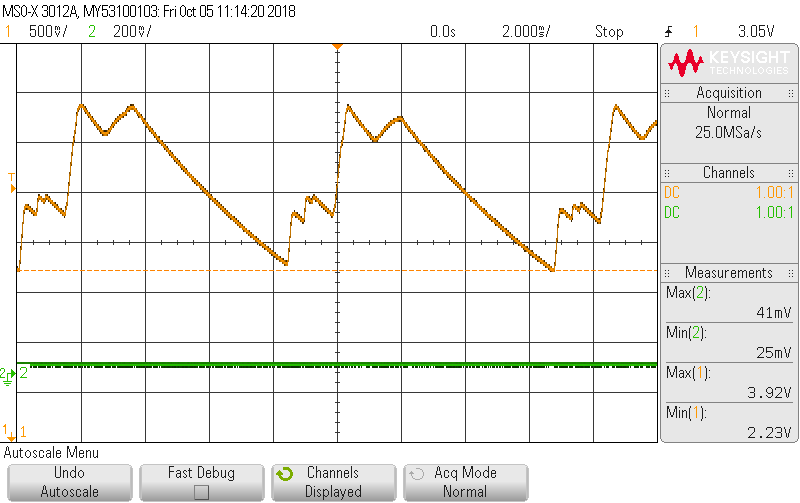
\includegraphics[width=0.9\textwidth]{figures/Osc-rectified.png}
\caption{Rectifier output comparison between black and white light.}
\end{figure}

\begin{figure}[H]
\centering
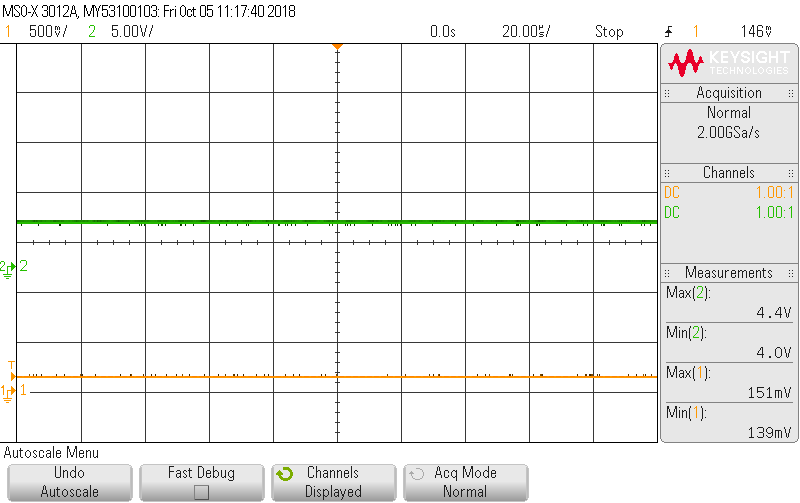
\includegraphics[width=0.9\textwidth]{figures/Osc-out.png}
\caption{Schmitt-trigger output comparison between black and white light.}
\end{figure}

\subsection*{Appendix: F}

\begin{figure}[H]
\centering
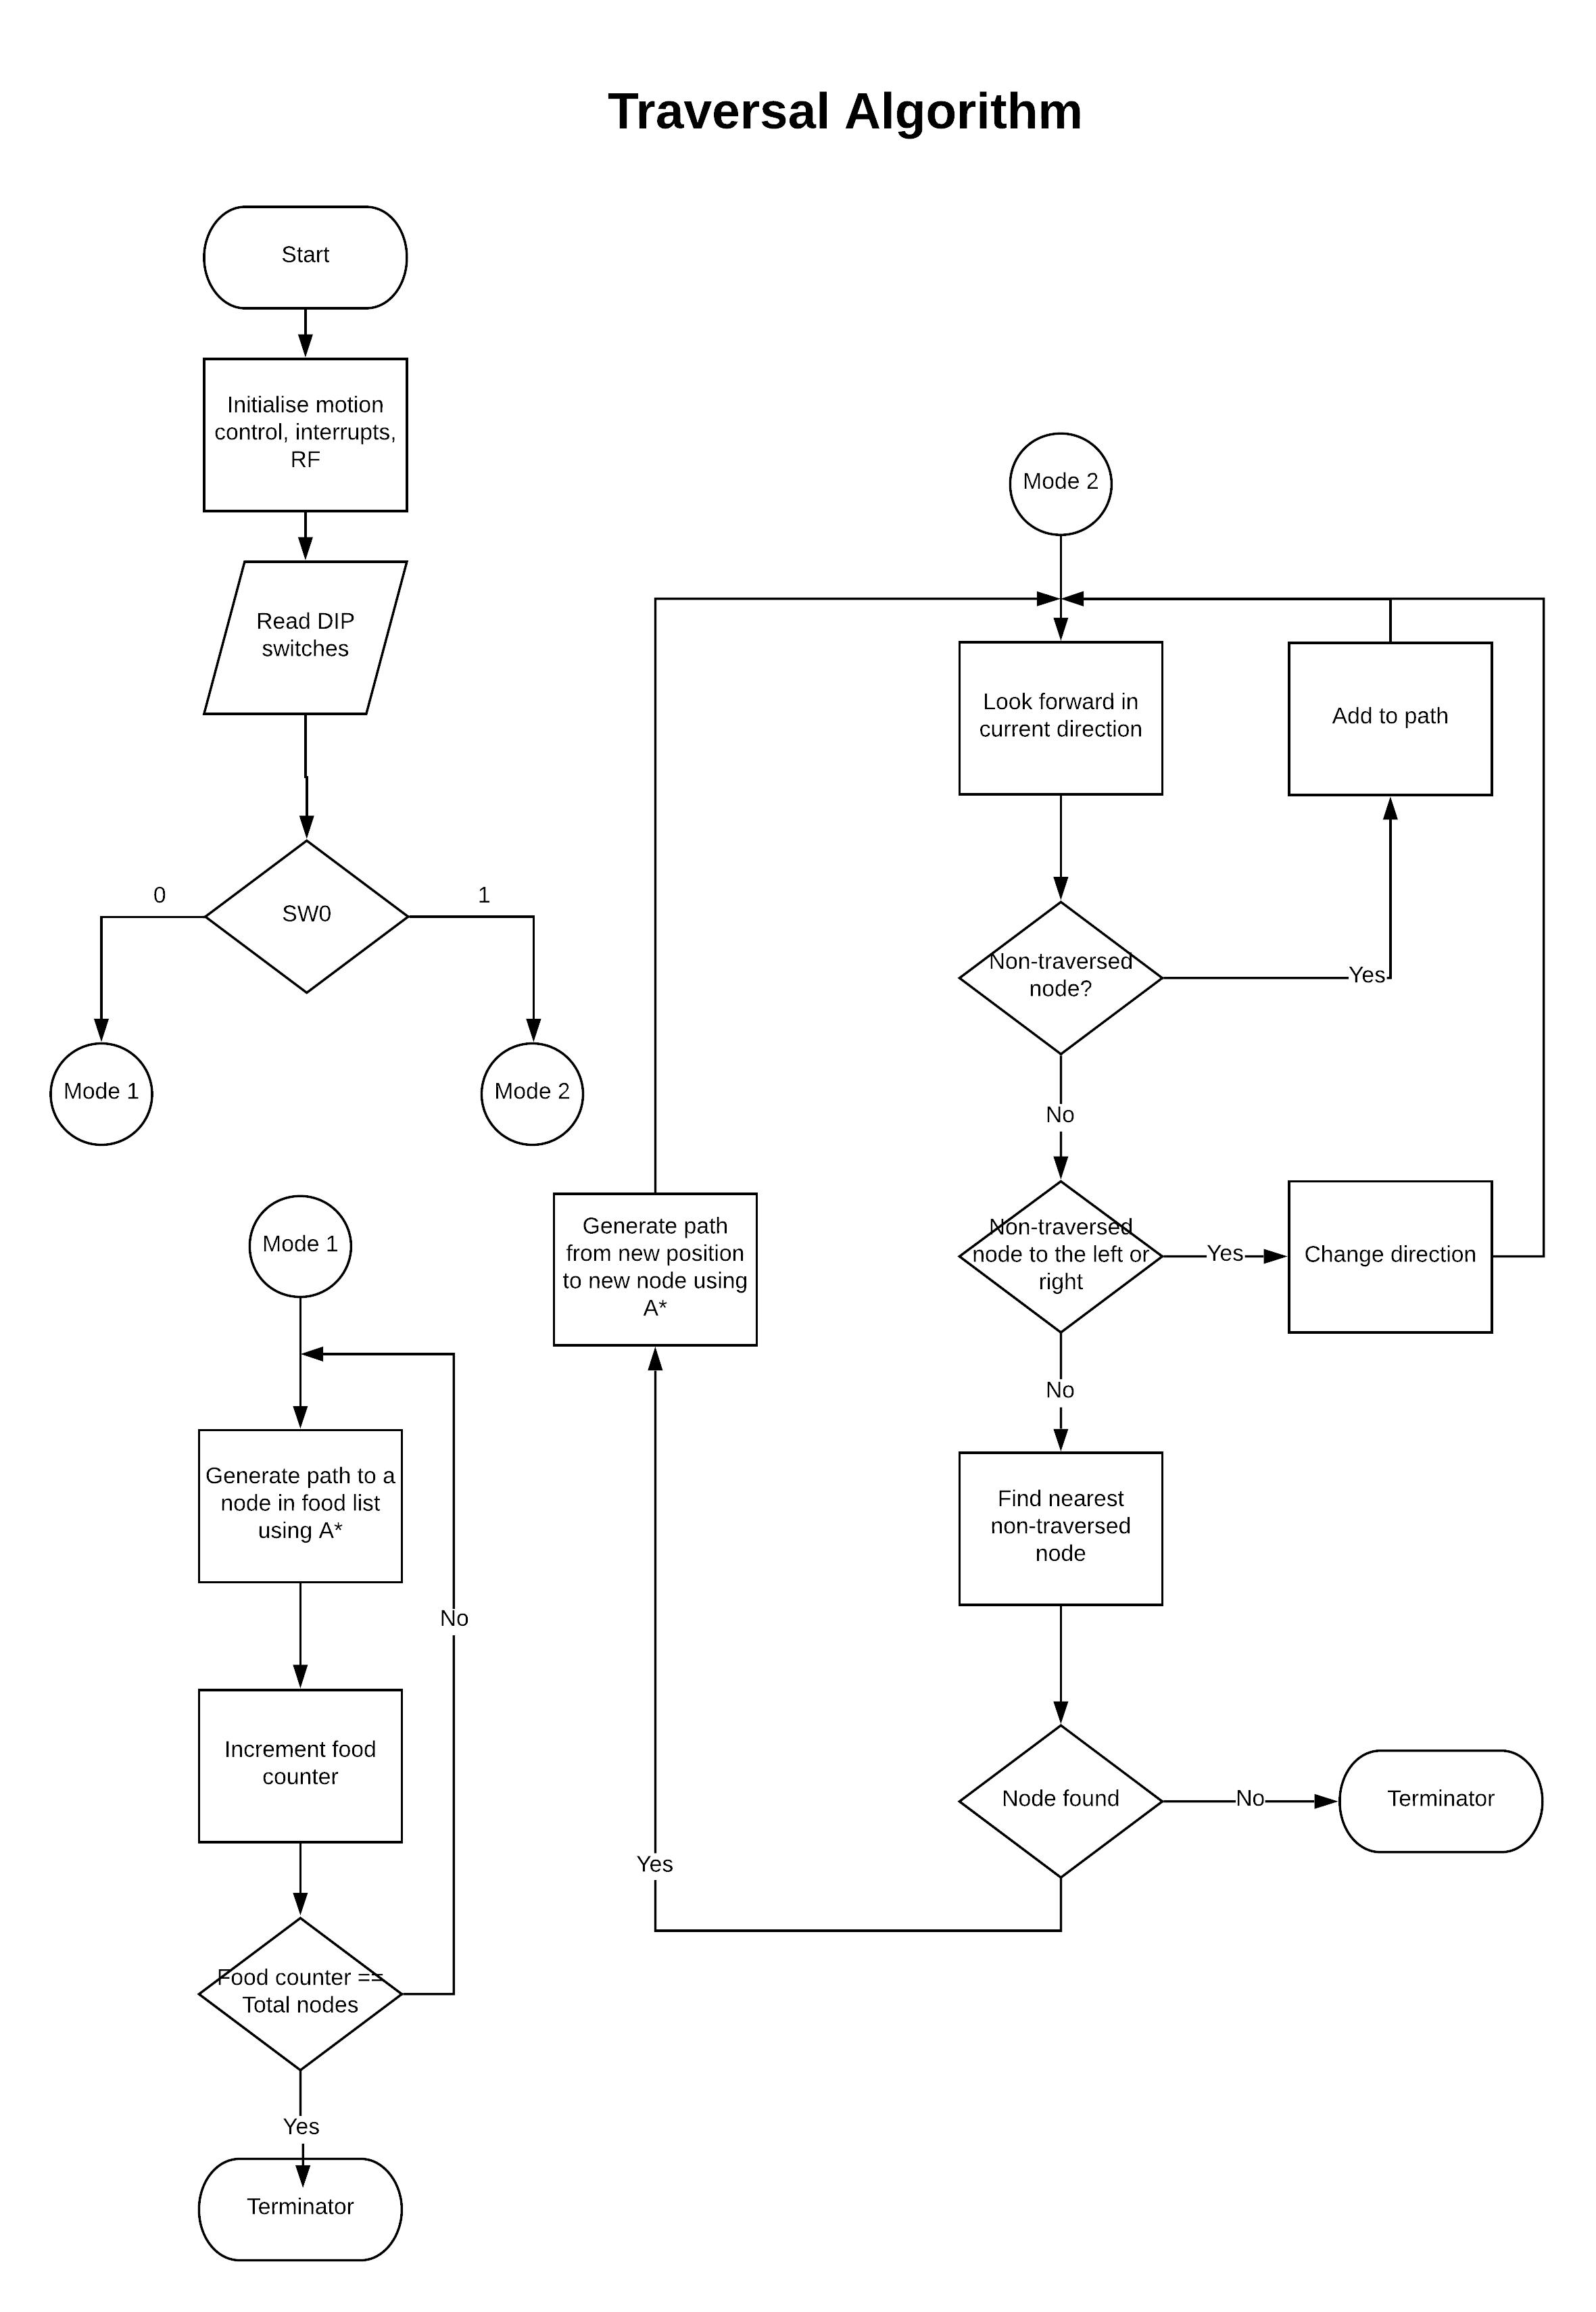
\includegraphics[width=0.8\textwidth]{figures/traverse_flowchart.png}
\caption{Traversal Algorithm Flowchart.}
\end{figure}

\begin{figure}[H]
\centering
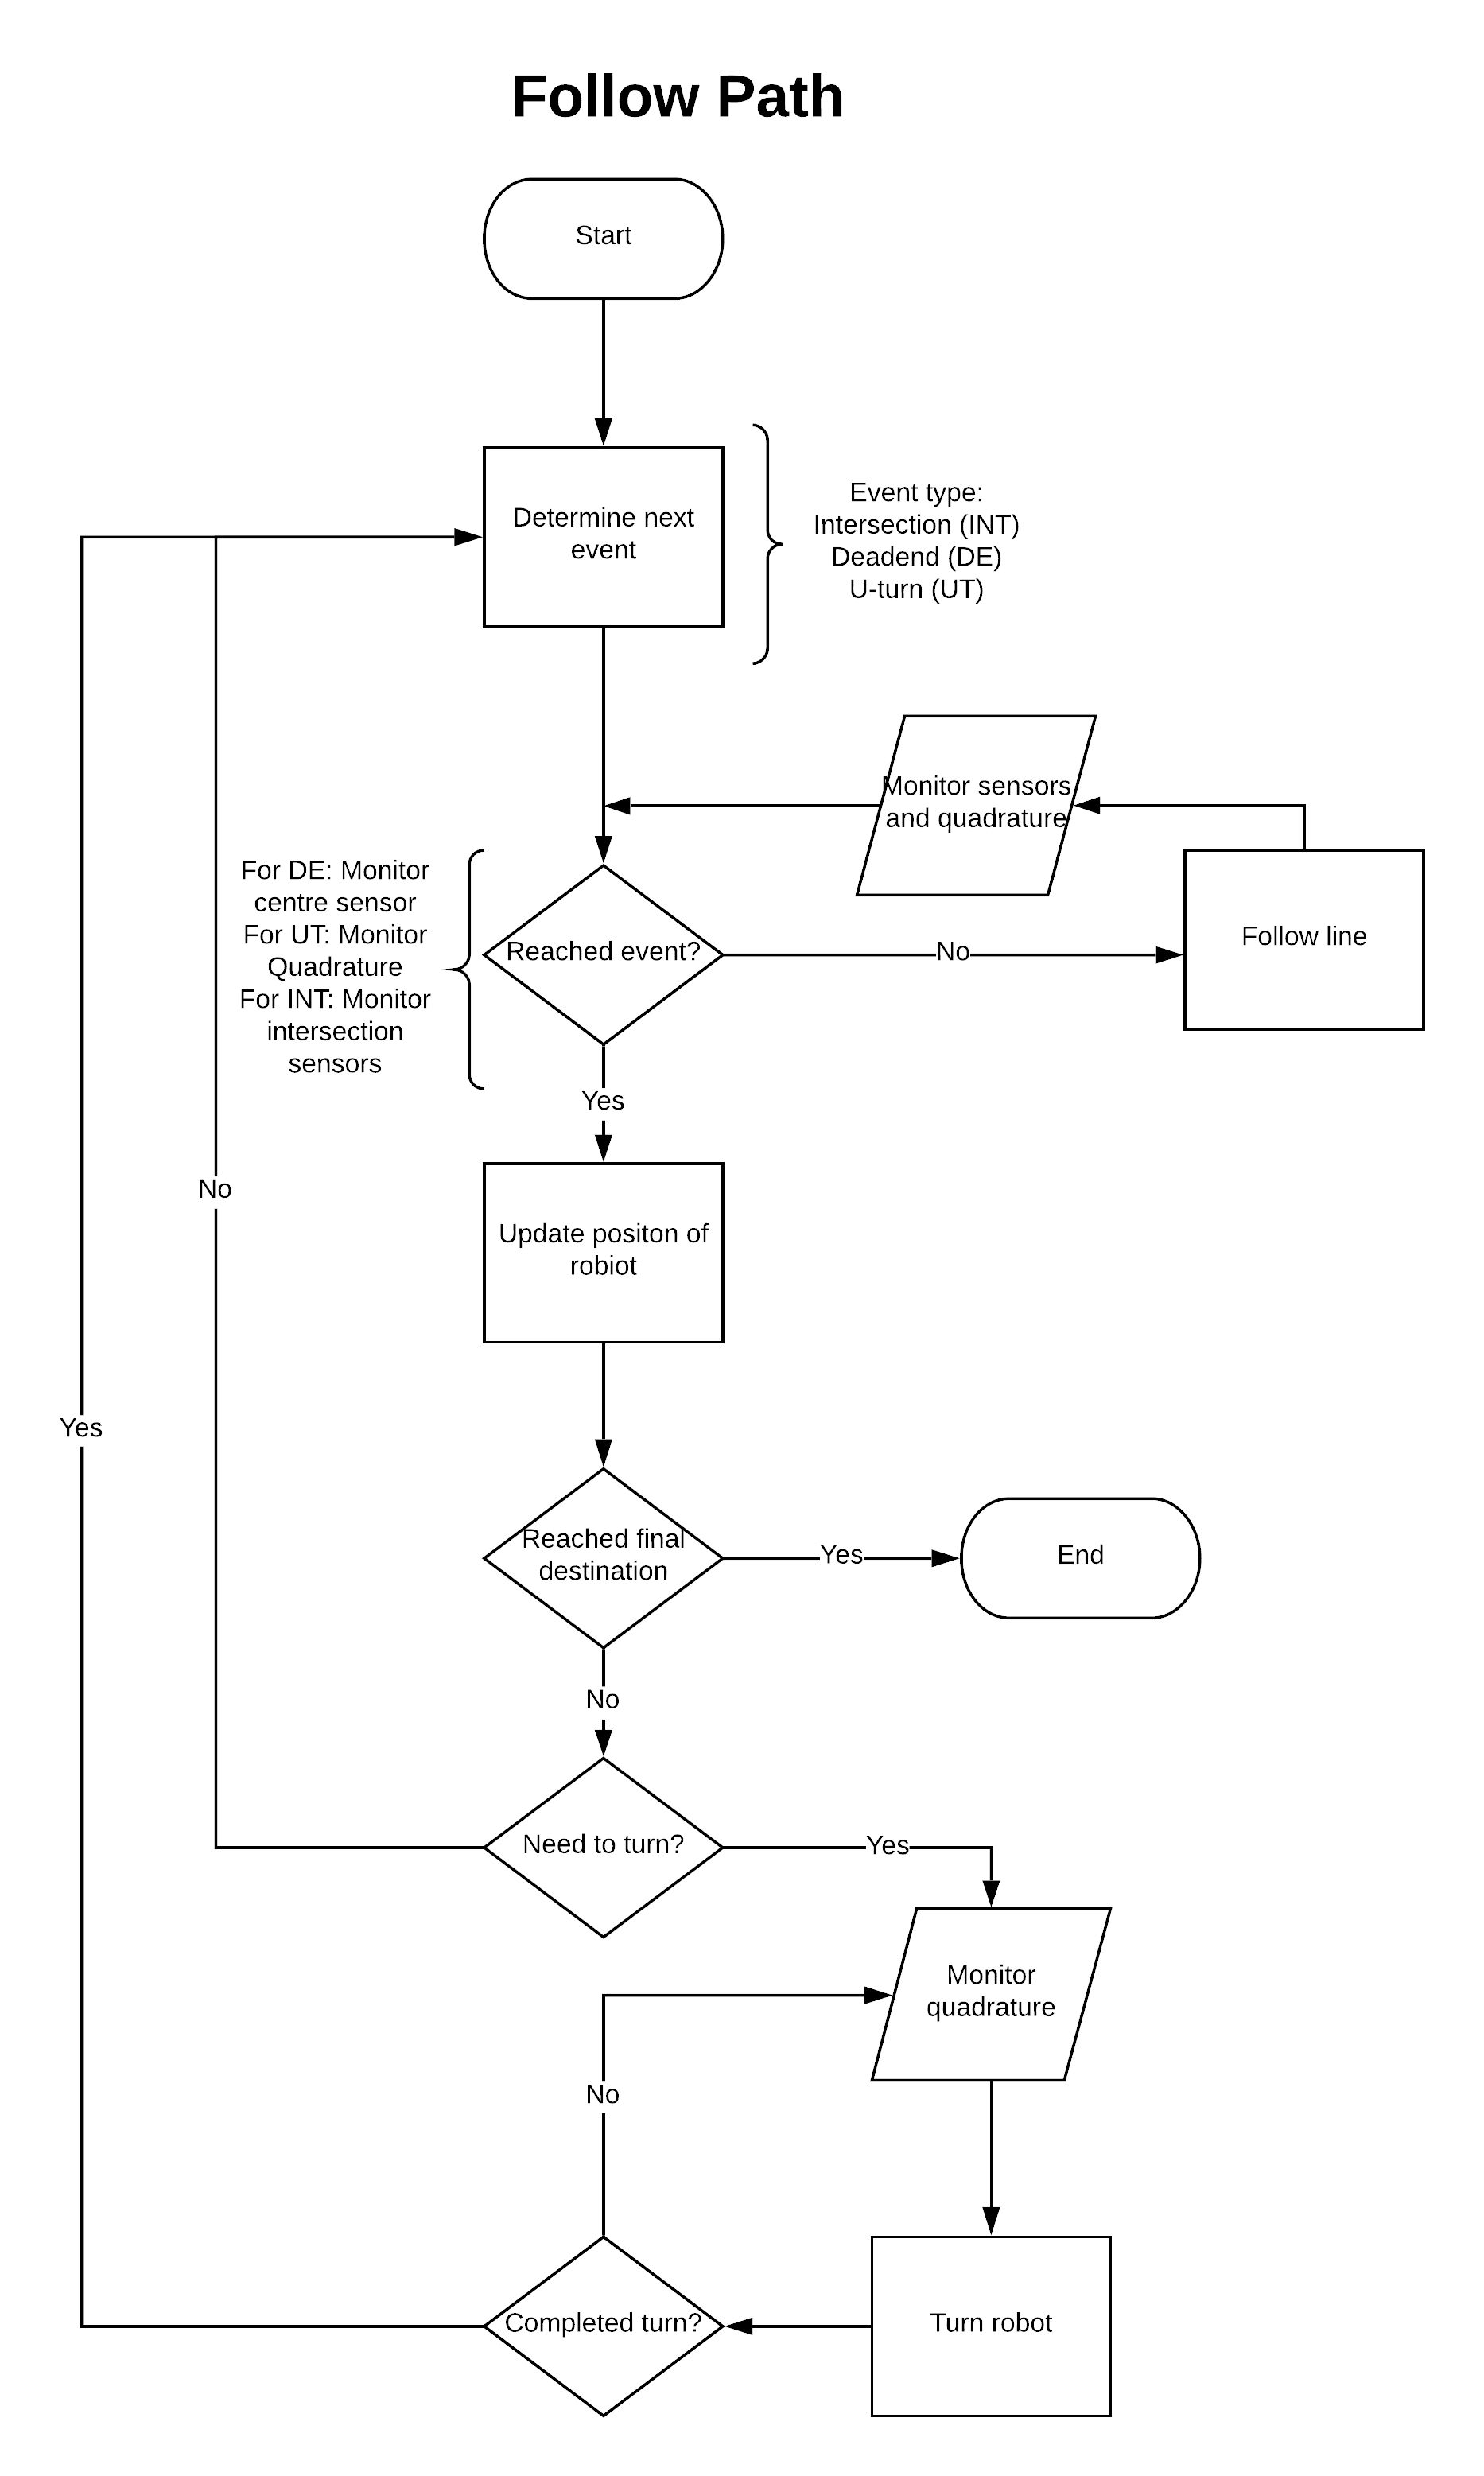
\includegraphics[width=0.7\textwidth]{figures/followpath_flowchart.png}
\caption{Follow Path Flowchart.}
\end{figure}

\begin{figure}[H]
\centering
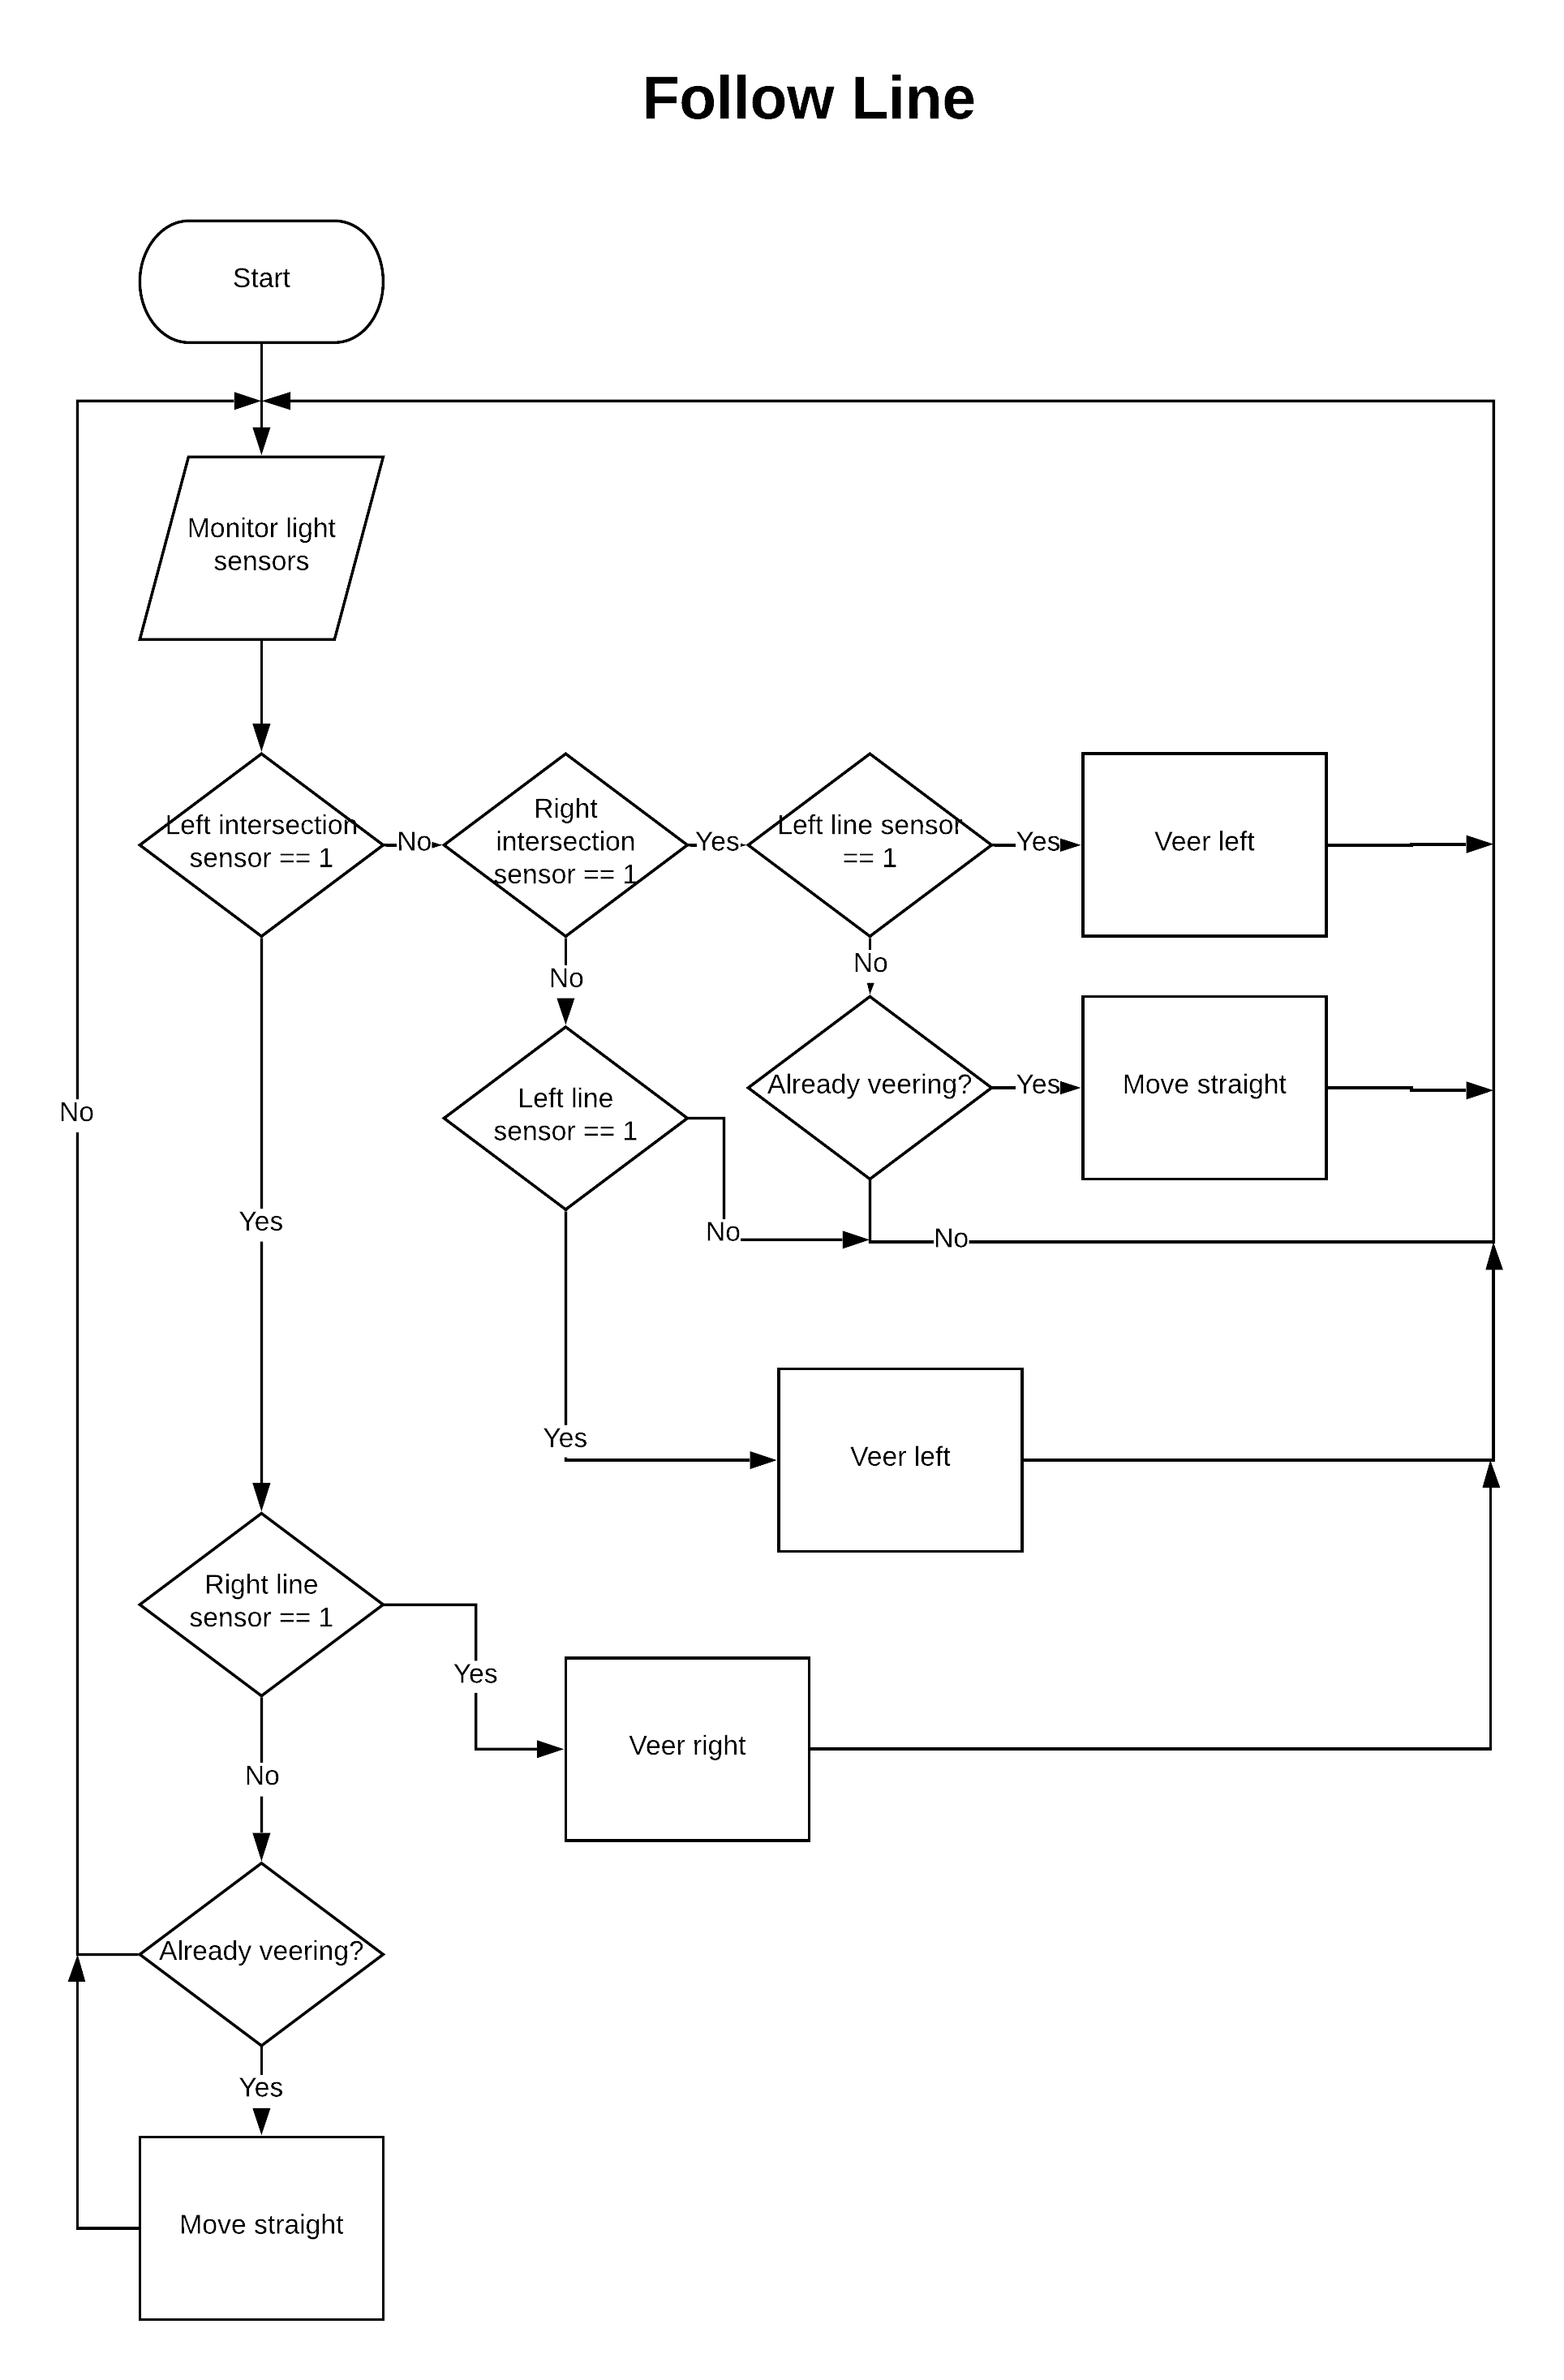
\includegraphics[width=0.8\textwidth]{figures/followline_flowchart.png}
\caption{Follow Line Flowchart.}
\end{figure}

\begin{figure}[H]
\centering
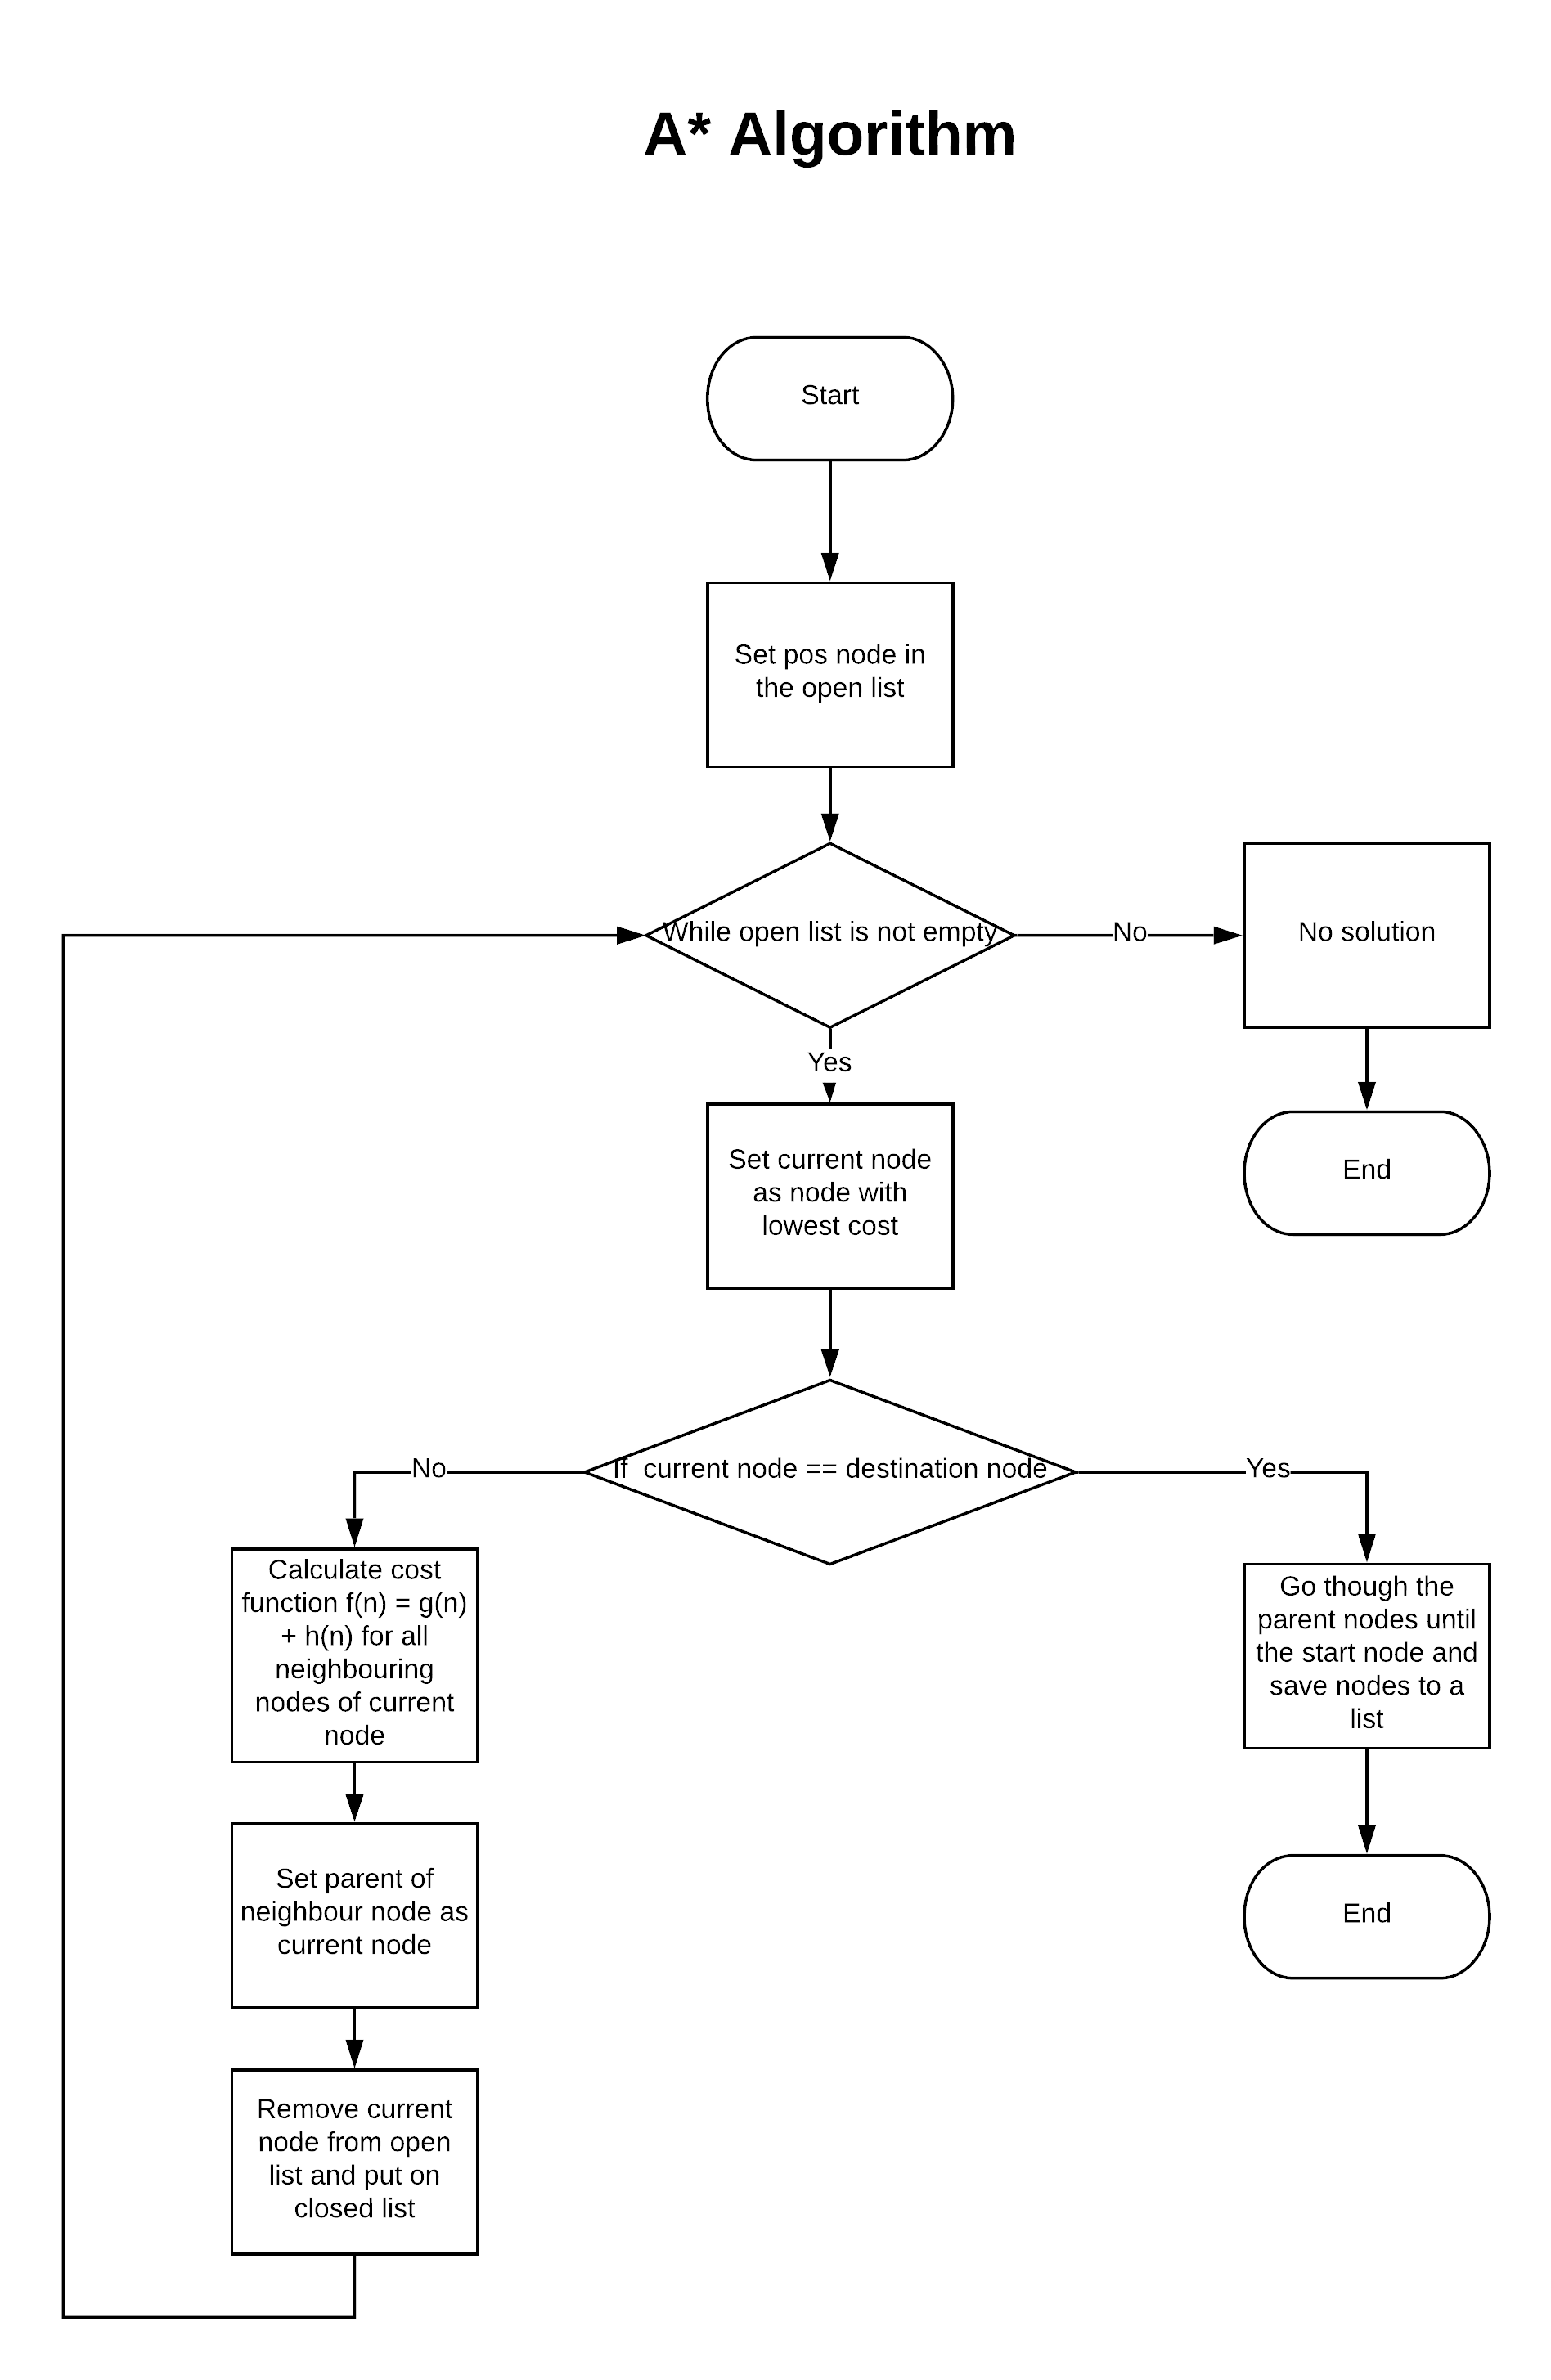
\includegraphics[width=0.8\textwidth]{figures/astar_flowchart.png}
\caption{A* Star Algorithm Flowchart.}
\end{figure}
\newpage
\section{Datasheet}
\vspace{1mm}
\Large \textbf{ADLQ - Line Following Robot Datasheet}

\begin{multicols}{2}

\subsection*{Product Overview}
\vspace{-2mm}
The ADLQ is a robot that follows black lines on a white background which has two modes. Mode One traverses a projected map whereas Mode Two finds the shortest path to a list of food pellets using A* algorithm. The modes can be changed using the onboard DIP switches. For optimal performance the robot’s operating voltage needs to be between 7.5 volts and 7.9 volts. ADLQ needs 6x1.2V batteries for operation.

\begin{figure}[H]
\centering
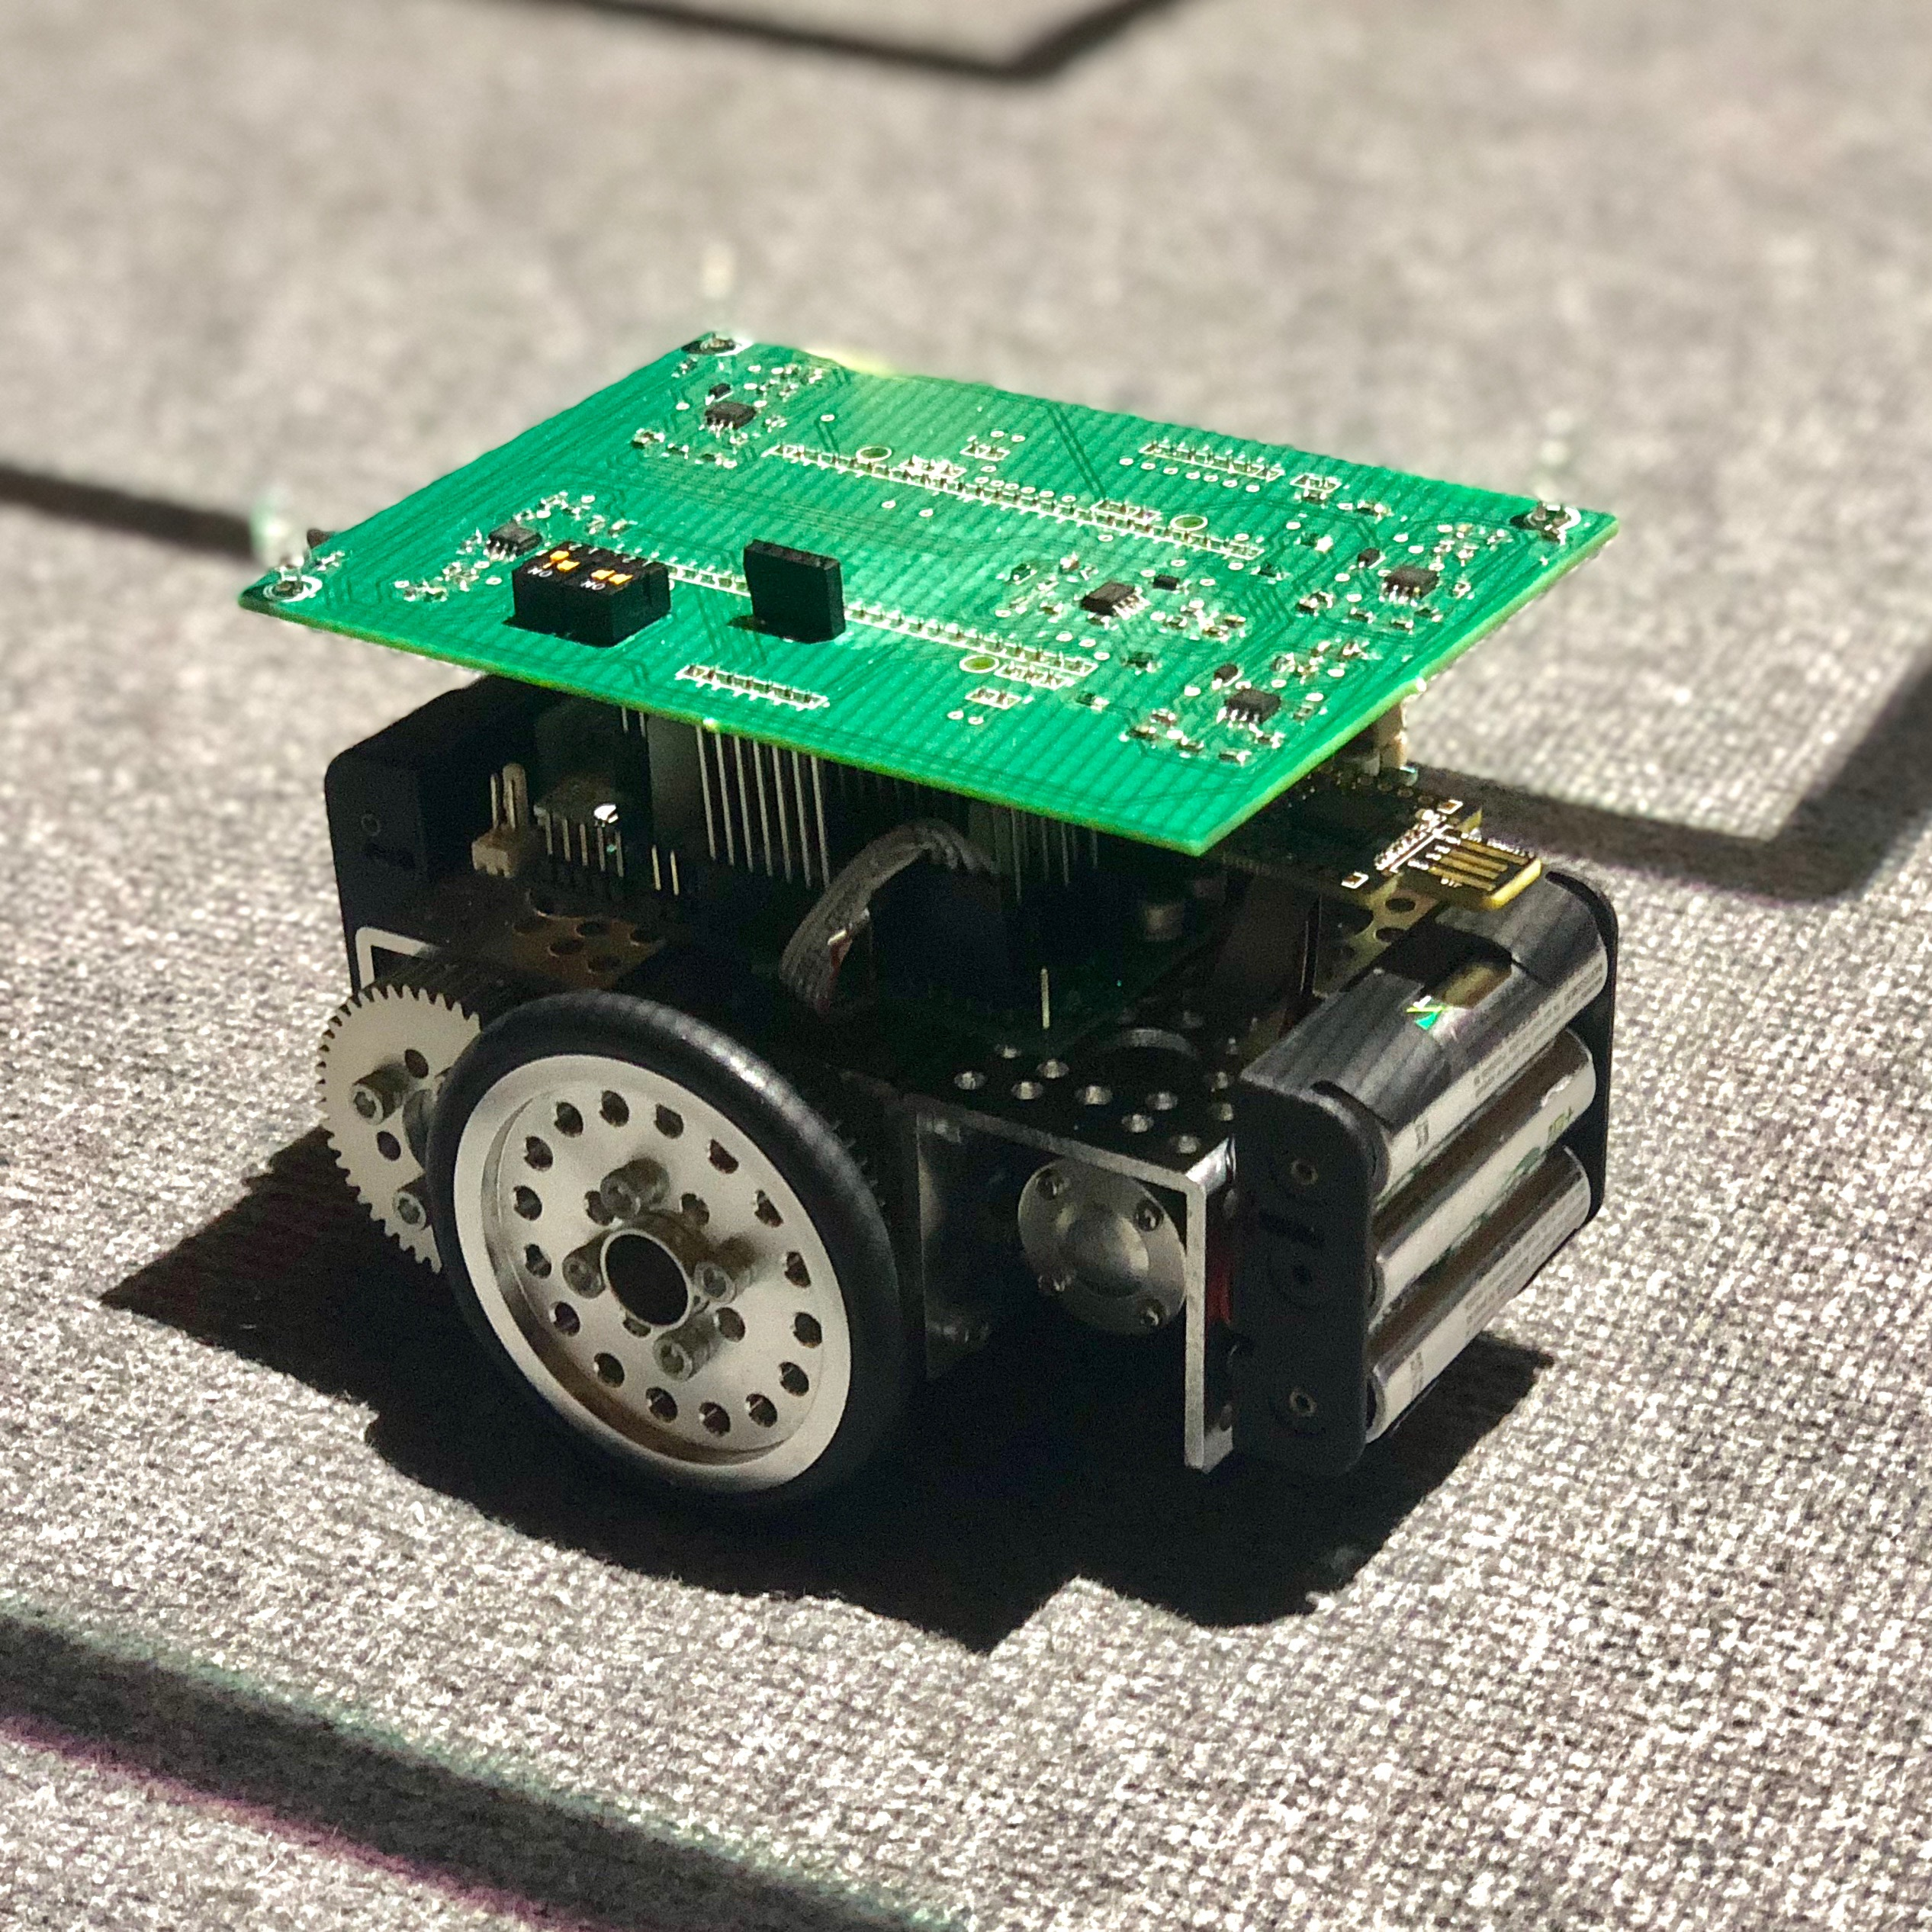
\includegraphics[width=0.4\textwidth]{figures/robot_img.JPG}
% \caption{BACK VIEW}
\end{figure}
\end{multicols}


\begin{multicols}{2}
\subsection*{Features}
\begin{itemize}
    \item 2 different modes:
    \begin{itemize}
        \item Traverse the map
        \item Shortest path
    \end{itemize}
    \item Travel Speed Range: 13-28cms\textsuperscript{-1}
\end{itemize}

\subsection*{Mode Selection}
The robot’s LEDs and mode configured using the onboard DIP switches. To enable the the LEDS, switch the left DIP switch 1 to ON. To enable the motors, switch the left DIP switch 2 to ON. For Mode 1 switch the right DIP switch 1 to ON and for Mode 2 switch the right DIP switch 1 to OFF.


\end{multicols}

\subsection*{Specifications}
\vspace{-4mm}
\begin{table}[h!]
\centering
\small
\resizebox{\textwidth}{!}{\begin{tabular}{|l|l|l|l|}
\hline
\textbf{PARAMETER} & \textbf{MIN} & \textbf{MAX} & \textbf{UNIT} \\ \hline
\textbf{\textit{Operating Voltage}} & 6.8 & 8.2 &   V                    \\ \hline
\textbf{\textit{Travel Speed}} & 13 & 28  & cms\textsuperscript{-1}      \\ \hline
\textbf{\textit{Line Detection Speed}} & 21 & 26 &   ms                   \\ \hline
\textbf{\textit{Wall Detection Speed}} & 14 & 19 &    ms                  \\ \hline
\textbf{\textit{Optimal Line Thickness}} & 18 & 22 &   mm                 \\ \hline
\textbf{\textit{Sensor Array Layout}} & \multicolumn{3}{l|}{2 left sensors, 2 right sensors and 1 centre sensor}             \\ \hline
\end{tabular}}
\end{table}

\subsection*{Robot Dimensions}
\vspace{-3mm}
\begin{figure}[H]
\centering
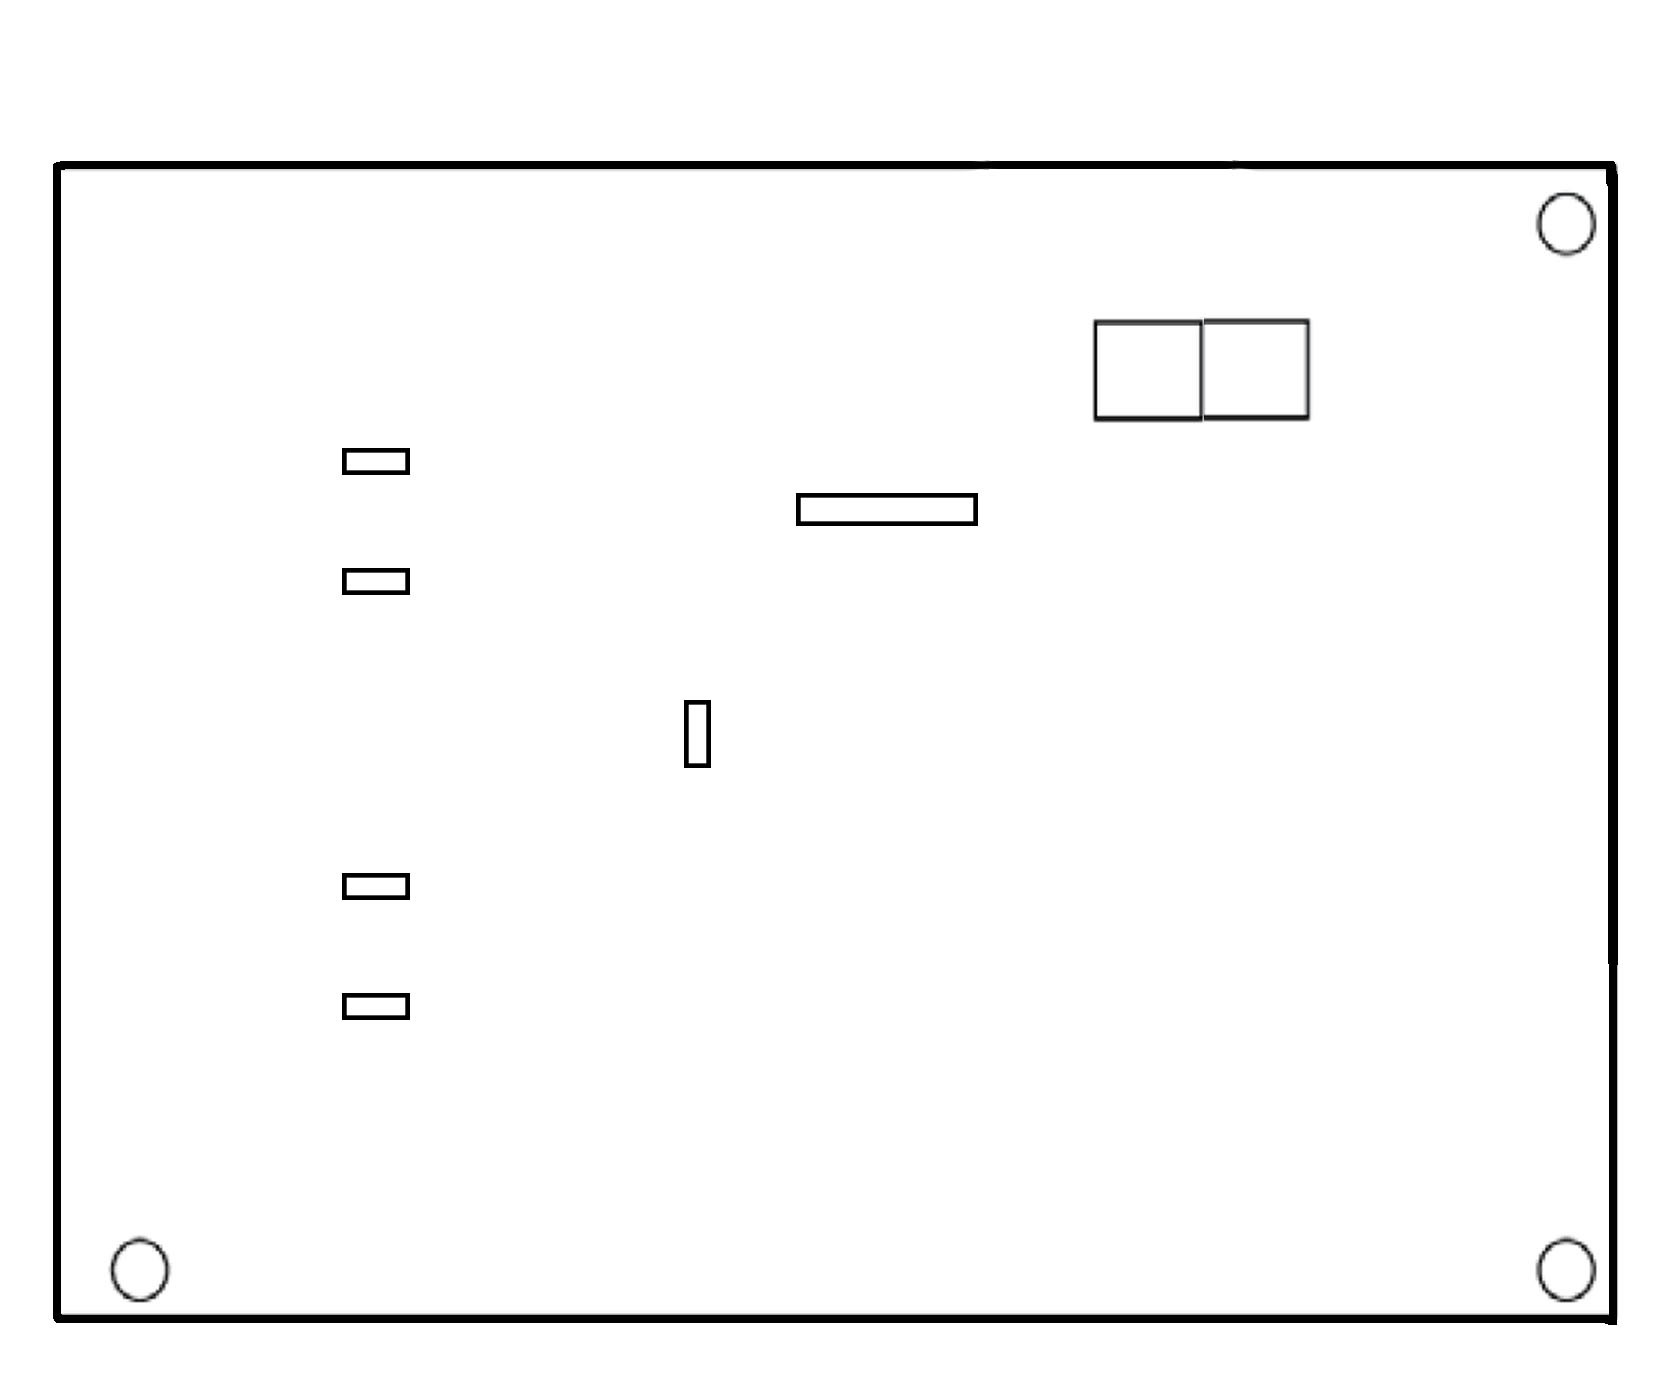
\includegraphics[width=0.39\textwidth]{figures/top_view.jpg}
\caption{TOP VIEW}
\end{figure}

\begin{figure}[H]
\centering
\hspace{-5mm}
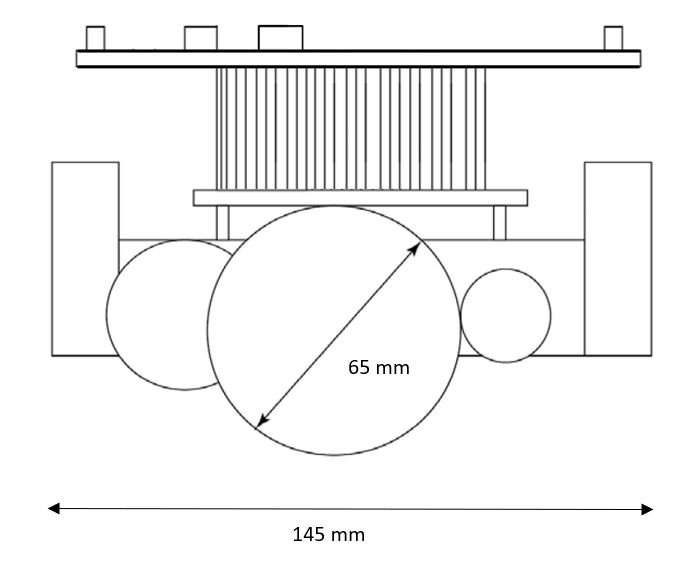
\includegraphics[width=0.45\textwidth]{figures/side_view.JPG}
\caption{SIDE VIEW}
\end{figure}

\begin{figure}[H]
\centering
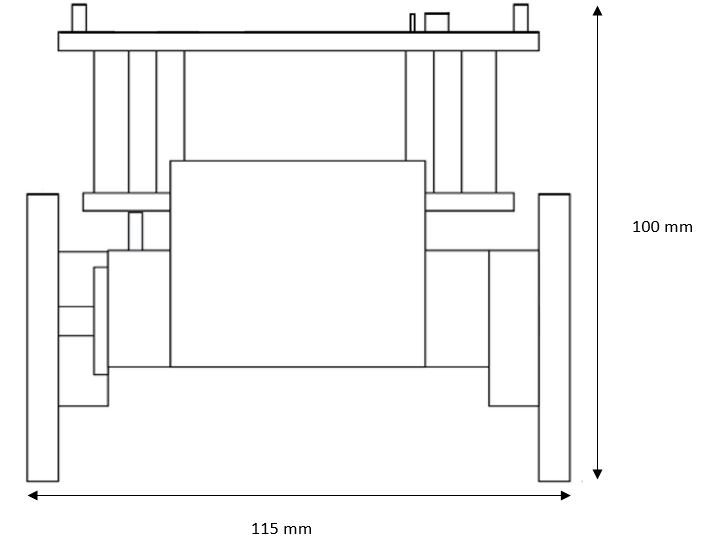
\includegraphics[width=0.42\textwidth]{figures/back_view.JPG}
\caption{BACK VIEW}
\end{figure}

% \newpage
% \bibliography{mybib}


\end{document}
%%% Local Variables: 
%%% mode: latex
%%% TeX-master: t
%%% End: 
